\documentclass[10pt,journal]{IEEEtran}
\usepackage{amsmath,amssymb}
\usepackage{booktabs}
\usepackage{graphicx}
\usepackage{microtype}
\usepackage{cite}
\usepackage{xspace}
\PassOptionsToPackage{hyphens}{url}
\usepackage{hyperref}
\Urlmuskip=0mu plus 2mu\relax
\emergencystretch=2em
\graphicspath{{../figures/}{./figures/}}
\renewcommand{\arraystretch}{1.15}
\setcounter{topnumber}{3}
\setcounter{bottomnumber}{2}
\setcounter{totalnumber}{4}
\renewcommand{\topfraction}{0.92}
\renewcommand{\bottomfraction}{0.75}
\renewcommand{\textfraction}{0.07}
\renewcommand{\floatpagefraction}{0.72}
\renewcommand{\dbltopfraction}{0.92}
\renewcommand{\dblfloatpagefraction}{0.72}

% Generated by code/make_manuscript_numbers.py -- do not edit by hand.
\newcommand{\BenchAmbiguous}{13}
\newcommand{\BenchCorrectPmg}{48}
\newcommand{\BenchCorrectVone}{51}
\newcommand{\BenchCorrectVoneFb}{51}
\newcommand{\BenchCorrectVtwo}{50}
\newcommand{\BenchCorrectVtwoGr}{50}
\newcommand{\BenchExactPmg}{38}
\newcommand{\BenchExactVone}{38}
\newcommand{\BenchExactVoneFb}{38}
\newcommand{\BenchExactVtwo}{37}
\newcommand{\BenchExactVtwoGr}{37}
\newcommand{\BenchFalseRefPmg}{0}
\newcommand{\BenchFalseRefVone}{0}
\newcommand{\BenchFalseRefVoneFb}{0}
\newcommand{\BenchFalseRefVtwo}{1}
\newcommand{\BenchFalseRefVtwoGr}{1}
\newcommand{\BenchResolvable}{38}
\newcommand{\BenchSilentPmg}{3}
\newcommand{\BenchSilentVone}{0}
\newcommand{\BenchSilentVoneFb}{0}
\newcommand{\BenchSilentVtwo}{0}
\newcommand{\BenchSilentVtwoGr}{0}
\newcommand{\DevAgreePctPmg}{84.6}
\newcommand{\DevAgreePctVone}{84.6}
\newcommand{\DevAgreePctVoneFb}{83.5}
\newcommand{\DevAgreePctVtwo}{87.2}
\newcommand{\DevAgreePctVtwoGr}{87.2}
\newcommand{\DevAgreePmg}{6{,}387}
\newcommand{\DevAgreeVone}{6{,}387}
\newcommand{\DevAgreeVoneFb}{6{,}303}
\newcommand{\DevAgreeVtwo}{6{,}588}
\newcommand{\DevAgreeVtwoGr}{6{,}588}
\newcommand{\DevBackendDisagree}{0}
\newcommand{\DevCost}{28}
\newcommand{\DevCostAt}{7}
\newcommand{\DevCostDot}{3}
\newcommand{\DevCostGroup}{5}
\newcommand{\DevCostHydrate}{0}
\newcommand{\DevCostOther}{0}
\newcommand{\DevCostSpace}{13}
\newcommand{\DevDiscExDummyPmg}{22}
\newcommand{\DevDiscExDummyVone}{22}
\newcommand{\DevDiscExDummyVoneFb}{8}
\newcommand{\DevDiscExDummyVtwo}{6}
\newcommand{\DevDiscExDummyVtwoGr}{6}
\newcommand{\DevDiscPmg}{399}
\newcommand{\DevDiscVone}{22}
\newcommand{\DevDiscVoneFb}{8}
\newcommand{\DevDiscVtwo}{6}
\newcommand{\DevDiscVtwoGr}{6}
\newcommand{\DevDummyPmg}{377}
\newcommand{\DevDummyVone}{0}
\newcommand{\DevDummyVoneFb}{0}
\newcommand{\DevDummyVtwo}{0}
\newcommand{\DevDummyVtwoGr}{0}
\newcommand{\DevGrammarOnly}{229}
\newcommand{\DevMcAgreePmgA}{229}
\newcommand{\DevMcAgreePmgB}{28}
\newcommand{\DevMcAgreePmgP}{<10^{-39}}
\newcommand{\DevMcAgreePmgPDoi}{<10^{-34}}
\newcommand{\DevMcAgreeVoneA}{229}
\newcommand{\DevMcAgreeVoneB}{28}
\newcommand{\DevMcAgreeVoneP}{<10^{-39}}
\newcommand{\DevMcAgreeVonePDoi}{<10^{-34}}
\newcommand{\DevMcDiscExDummyPmgA}{0}
\newcommand{\DevMcDiscExDummyPmgB}{16}
\newcommand{\DevMcDiscExDummyPmgP}{<10^{-4}}
\newcommand{\DevMcDiscExDummyPmgPDoi}{<10^{-4}}
\newcommand{\DevMcDiscExDummyVoneA}{0}
\newcommand{\DevMcDiscExDummyVoneB}{16}
\newcommand{\DevMcDiscExDummyVoneP}{<10^{-4}}
\newcommand{\DevMcDiscExDummyVonePDoi}{<10^{-4}}
\newcommand{\DevMcDiscPmgA}{0}
\newcommand{\DevMcDiscPmgB}{393}
\newcommand{\DevMcDiscPmgP}{<10^{-118}}
\newcommand{\DevMcDiscPmgPDoi}{<10^{-111}}
\newcommand{\DevMcDiscVoneA}{0}
\newcommand{\DevMcDiscVoneB}{16}
\newcommand{\DevMcDiscVoneP}{<10^{-4}}
\newcommand{\DevMcDiscVonePDoi}{<10^{-4}}
\newcommand{\DevMixAgree}{163}
\newcommand{\DevMixDisagree}{2}
\newcommand{\DevMixRefused}{1{,}208}
\newcommand{\DevReasonElVar}{801}
\newcommand{\DevReasonFreeCoef}{1{,}208}
\newcommand{\DevReasonFreeVar}{5{,}633}
\newcommand{\DevReasonOxDef}{2{,}090}
\newcommand{\DevReasonUnqDopant}{773}
\newcommand{\DevReasonZeroAmt}{13}
\newcommand{\DevRefusedPmg}{1{,}137}
\newcommand{\DevRefusedVone}{1{,}155}
\newcommand{\DevRefusedVoneFb}{1{,}245}
\newcommand{\DevRefusedVtwo}{962}
\newcommand{\DevRefusedVtwoGr}{962}
\newcommand{\HoAgreePctPmg}{78.3}
\newcommand{\HoAgreePctVone}{78.1}
\newcommand{\HoAgreePctVoneFb}{75.3}
\newcommand{\HoAgreePctVtwo}{78.3}
\newcommand{\HoAgreePctVtwoGr}{78.3}
\newcommand{\HoAgreePmg}{1{,}098}
\newcommand{\HoAgreeVone}{1{,}096}
\newcommand{\HoAgreeVoneFb}{1{,}056}
\newcommand{\HoAgreeVtwo}{1{,}099}
\newcommand{\HoAgreeVtwoGr}{1{,}099}
\newcommand{\HoBackendDisagree}{0}
\newcommand{\HoCost}{33}
\newcommand{\HoCostAt}{18}
\newcommand{\HoCostDot}{0}
\newcommand{\HoCostGroup}{3}
\newcommand{\HoCostHydrate}{2}
\newcommand{\HoCostOther}{1}
\newcommand{\HoCostSpace}{9}
\newcommand{\HoDiscExDummyPmg}{5}
\newcommand{\HoDiscExDummyVone}{5}
\newcommand{\HoDiscExDummyVoneFb}{3}
\newcommand{\HoDiscExDummyVtwo}{3}
\newcommand{\HoDiscExDummyVtwoGr}{3}
\newcommand{\HoDiscPmg}{53}
\newcommand{\HoDiscVone}{5}
\newcommand{\HoDiscVoneFb}{3}
\newcommand{\HoDiscVtwo}{3}
\newcommand{\HoDiscVtwoGr}{3}
\newcommand{\HoDummyPmg}{48}
\newcommand{\HoDummyVone}{0}
\newcommand{\HoDummyVoneFb}{0}
\newcommand{\HoDummyVtwo}{0}
\newcommand{\HoDummyVtwoGr}{0}
\newcommand{\HoGrammarOnly}{34}
\newcommand{\HoMcAgreePmgA}{34}
\newcommand{\HoMcAgreePmgB}{33}
\newcommand{\HoMcAgreePmgP}{=1.00}
\newcommand{\HoMcAgreePmgPDoi}{=0.80}
\newcommand{\HoMcAgreeVoneA}{34}
\newcommand{\HoMcAgreeVoneB}{31}
\newcommand{\HoMcAgreeVoneP}{=0.80}
\newcommand{\HoMcAgreeVonePDoi}{=1.00}
\newcommand{\HoMcDiscExDummyPmgA}{0}
\newcommand{\HoMcDiscExDummyPmgB}{2}
\newcommand{\HoMcDiscExDummyPmgP}{=0.50}
\newcommand{\HoMcDiscExDummyPmgPDoi}{=0.50}
\newcommand{\HoMcDiscExDummyVoneA}{0}
\newcommand{\HoMcDiscExDummyVoneB}{2}
\newcommand{\HoMcDiscExDummyVoneP}{=0.50}
\newcommand{\HoMcDiscExDummyVonePDoi}{=0.50}
\newcommand{\HoMcDiscPmgA}{0}
\newcommand{\HoMcDiscPmgB}{50}
\newcommand{\HoMcDiscPmgP}{<10^{-14}}
\newcommand{\HoMcDiscPmgPDoi}{<10^{-14}}
\newcommand{\HoMcDiscVoneA}{0}
\newcommand{\HoMcDiscVoneB}{2}
\newcommand{\HoMcDiscVoneP}{=0.50}
\newcommand{\HoMcDiscVonePDoi}{=0.50}
\newcommand{\HoMixAgree}{18}
\newcommand{\HoMixDisagree}{0}
\newcommand{\HoMixRefused}{214}
\newcommand{\HoReasonElVar}{116}
\newcommand{\HoReasonFreeCoef}{61}
\newcommand{\HoReasonFreeVar}{968}
\newcommand{\HoReasonOxDef}{631}
\newcommand{\HoReasonUnqDopant}{111}
\newcommand{\HoReasonZeroAmt}{2}
\newcommand{\HoRefusedPmg}{295}
\newcommand{\HoRefusedVone}{302}
\newcommand{\HoRefusedVoneFb}{344}
\newcommand{\HoRefusedVtwo}{301}
\newcommand{\HoRefusedVtwoGr}{301}
\newcommand{\NAnnotation}{304}
\newcommand{\NBench}{51}
\newcommand{\NCorpus}{28{,}100}
\newcommand{\NCorpusCrossDataset}{2{,}070}
\newcommand{\NCorpusDatasets}{6}
\newcommand{\NCorpusDecimal}{0}
\newcommand{\NCorpusDistinct}{24{,}672}
\newcommand{\NCorpusParen}{205}
\newcommand{\NCorpusReduced}{14{,}147}
\newcommand{\NDevDOIs}{16{,}225}
\newcommand{\NDevDet}{7{,}552}
\newcommand{\NDevIndet}{10{,}518}
\newcommand{\NDevMix}{1{,}373}
\newcommand{\NDevStrings}{19{,}443}
\newcommand{\NDiel}{964}
\newcommand{\NDielInSharedSystems}{147}
\newcommand{\NDielReduced}{964}
\newcommand{\NDielSharedSystems}{69}
\newcommand{\NDielSystems}{886}
\newcommand{\NFlags}{15}
\newcommand{\NHazClasses}{8}
\newcommand{\NHazDev}{421}
\newcommand{\NHazHo}{83}
\newcommand{\NHazVone}{77}
\newcommand{\NHoDOIs}{3{,}039}
\newcommand{\NHoDet}{1{,}403}
\newcommand{\NHoDoiInDev}{65}
\newcommand{\NHoIndet}{1{,}889}
\newcommand{\NHoMix}{232}
\newcommand{\NHoStrings}{3{,}524}
\newcommand{\NLitDOIs}{19{,}234}
\newcommand{\NLitStrings}{22{,}967}
\newcommand{\NRemovedRuleCorpus}{52}
\newcommand{\NSeed}{27}
\newcommand{\NStress}{24}
\newcommand{\NStressFamilies}{16}
\newcommand{\NVtwoDiscTotal}{9}
\newcommand{\ParserVersion}{0.2.0}
\newcommand{\PctCorpusParen}{0.73}

% Generated by make_stage_numbers.py from the result files listed in stage_numbers_sources.csv -- do not edit by hand.
\newcommand{\StOneDet}{1{,}403}
\newcommand{\StOneAgree}{1{,}170}
\newcommand{\StOneAgreePct}{83.4}
\newcommand{\StOneDisc}{3}
\newcommand{\StOneGainPmg}{72}
\newcommand{\StOneMcAPmg}{105}
\newcommand{\StOneMcBPmg}{33}
\newcommand{\StOnePPmg}{=6.1\times10^{-10}}
\newcommand{\StOneDoiAPmg}{94}
\newcommand{\StOneDoiBPmg}{32}
\newcommand{\StOnePDoiPmg}{=2.9\times10^{-8}}
\newcommand{\StOneDiffPmg}{5.13}
\newcommand{\StOneLoPmg}{3.51}
\newcommand{\StOneHiPmg}{6.82}
\newcommand{\StOneGainVone}{74}
\newcommand{\StOneMcAVone}{105}
\newcommand{\StOneMcBVone}{31}
\newcommand{\StOnePVone}{=1.3\times10^{-10}}
\newcommand{\StOneDoiAVone}{94}
\newcommand{\StOneDoiBVone}{30}
\newcommand{\StOnePDoiVone}{=7.1\times10^{-9}}
\newcommand{\StOneDiffVone}{5.27}
\newcommand{\StOneLoVone}{3.52}
\newcommand{\StOneHiVone}{6.99}
\newcommand{\StOneGainVtwo}{71}
\newcommand{\StOneMcAVtwo}{71}
\newcommand{\StOneMcBVtwo}{0}
\newcommand{\StOnePVtwo}{=8.5\times10^{-22}}
\newcommand{\StOneDoiAVtwo}{65}
\newcommand{\StOneDoiBVtwo}{0}
\newcommand{\StOnePDoiVtwo}{=5.4\times10^{-20}}
\newcommand{\StOneDiffVtwo}{5.06}
\newcommand{\StOneLoVtwo}{3.91}
\newcommand{\StOneHiVtwo}{6.31}
\newcommand{\StOneNewDiscA}{0}
\newcommand{\StOneRescued}{71}
\newcommand{\StOneRescuedAgree}{71}
\newcommand{\StOneWrong}{3}
\newcommand{\StOneUncertain}{2}
\newcommand{\StOneCorrect}{66}
\newcommand{\StOneRescuedOther}{45}
\newcommand{\StOneWrongPct}{4.2}
\newcommand{\StOneWrongLo}{1.4}
\newcommand{\StOneWrongHi}{11.7}
\newcommand{\StOneWrongUPct}{7.0}
\newcommand{\StOneWrongULo}{3.0}
\newcommand{\StOneWrongUHi}{15.4}
\newcommand{\StOneThreshold}{43}
\newcommand{\StTwoStrings}{5{,}555}
\newcommand{\StTwoDOIs}{3{,}942}
\newcommand{\StTwoDet}{3{,}452}
\newcommand{\StTwoMix}{1{,}879}
\newcommand{\StTwoIndet}{224}
\newcommand{\StTwoSolid}{3{,}277}
\newcommand{\StTwoSolgel}{2{,}278}
\newcommand{\StTwoAgreePmg}{1{,}499}
\newcommand{\StTwoAgreePctPmg}{43.4}
\newcommand{\StTwoDiscPmg}{72}
\newcommand{\StTwoAgreeVone}{1{,}419}
\newcommand{\StTwoAgreePctVone}{41.1}
\newcommand{\StTwoDiscVone}{23}
\newcommand{\StTwoAgreeVtwo}{1{,}429}
\newcommand{\StTwoAgreePctVtwo}{41.4}
\newcommand{\StTwoDiscVtwo}{61}
\newcommand{\StTwoAgreeStrip}{1{,}735}
\newcommand{\StTwoAgreePctStrip}{50.3}
\newcommand{\StTwoDiscStrip}{61}
\newcommand{\StTwoAgreeStage}{1{,}732}
\newcommand{\StTwoAgreePctStage}{50.2}
\newcommand{\StTwoDiscStage}{61}
\newcommand{\StTwoGainPmg}{233}
\newcommand{\StTwoMcAPmg}{318}
\newcommand{\StTwoMcBPmg}{85}
\newcommand{\StTwoPPmg}{=9.4\times10^{-33}}
\newcommand{\StTwoDoiAPmg}{227}
\newcommand{\StTwoDoiBPmg}{61}
\newcommand{\StTwoPDoiPmg}{=1.2\times10^{-23}}
\newcommand{\StTwoDiffPmg}{6.75}
\newcommand{\StTwoLoPmg}{5.35}
\newcommand{\StTwoHiPmg}{8.15}
\newcommand{\StTwoGainVone}{313}
\newcommand{\StTwoMcAVone}{318}
\newcommand{\StTwoMcBVone}{5}
\newcommand{\StTwoPVone}{=3.4\times10^{-87}}
\newcommand{\StTwoDoiAVone}{228}
\newcommand{\StTwoDoiBVone}{5}
\newcommand{\StTwoPDoiVone}{=8.1\times10^{-61}}
\newcommand{\StTwoDiffVone}{9.07}
\newcommand{\StTwoLoVone}{7.89}
\newcommand{\StTwoHiVone}{10.34}
\newcommand{\StTwoGainVtwo}{303}
\newcommand{\StTwoMcAVtwo}{303}
\newcommand{\StTwoMcBVtwo}{0}
\newcommand{\StTwoPVtwo}{=1.2\times10^{-91}}
\newcommand{\StTwoDoiAVtwo}{215}
\newcommand{\StTwoDoiBVtwo}{0}
\newcommand{\StTwoPDoiVtwo}{=3.8\times10^{-65}}
\newcommand{\StTwoDiffVtwo}{8.78}
\newcommand{\StTwoLoVtwo}{7.62}
\newcommand{\StTwoHiVtwo}{9.96}
\newcommand{\StTwoNewDiscA}{0}
\newcommand{\StTwoGuardCostB}{3}
\newcommand{\StTwoGuardCostP}{=0.25}
\newcommand{\StTwoThreshold}{104}
\newcommand{\StTwoGuardRefused}{3}
\newcommand{\StTwoRescued}{303}
\newcommand{\StTwoRescuedAgree}{303}
\newcommand{\StTwoSample}{200}
\newcommand{\StTwoWrong}{3}
\newcommand{\StTwoWrongPct}{1.5}
\newcommand{\StTwoWrongLo}{0.5}
\newcommand{\StTwoWrongHi}{4.3}
\newcommand{\StTwoWrongAll}{4}
\newcommand{\StTwoWrongAllPct}{1.3}
\newcommand{\StTwoWrongAllLo}{0.5}
\newcommand{\StTwoWrongAllHi}{3.3}
\newcommand{\StTwoSuspect}{1}
\newcommand{\GthreeTwoAgree}{1{,}728}
\newcommand{\GthreeTwoAgreePct}{50.1}
\newcommand{\GthreeOneAgree}{1{,}167}
\newcommand{\GuardOneAgree}{1{,}167}
\newcommand{\GthreeTwoGainPmg}{229}
\newcommand{\GthreeTwoDiffPmg}{6.63}
\newcommand{\GthreeTwoLoPmg}{5.27}
\newcommand{\GthreeTwoHiPmg}{8.01}
\newcommand{\GthreeTwoPPmg}{=5.8\times10^{-32}}
\newcommand{\GthreeTwoCost}{4}
\newcommand{\GthreeTwoCostP}{=0.125}
\newcommand{\GthreeTwoRefused}{4}
\newcommand{\GthreeOneRefused}{0}
\newcommand{\StDevHalf}{9{,}831}
\newcommand{\StDevTestHalf}{9{,}612}
\newcommand{\StDevHalfDet}{3{,}797}
\newcommand{\StDevTestHalfDet}{3{,}755}
\newcommand{\StTwoRescuedOther}{165}
\newcommand{\StTwoRescuedParen}{128}
\newcommand{\StTwoRescuedPmgRefused}{303}
\newcommand{\StOneRescuedPmgRefused}{71}
   % normalization-stage numbers, written by make_stage_numbers.py
\usepackage{xcolor}
\newcommand{\PENDING}[1]{\textcolor{red}{\textbf{[PENDING: #1]}}}
\newcommand{\pmg}{\texttt{pymatgen}\xspace}

%% ---------------------------------------------------------------------------
%% Author-action notes are kept in the source but not typeset.
\long\def\authoraction#1{}
%% ---------------------------------------------------------------------------
%% DEPOSIT DOI.  Set it in deposit_doi.tex (shared with esi.tex and the response
%% letter) and rebuild. Until then the text states, accurately,
%% that the versioned archive accompanies the submission and that no public
%% deposit exists yet; no string shaped like a DOI is printed.
% The ONE place to set the deposit DOI (e.g. 10.5281/zenodo.1234567). Read by main.tex,
% esi.tex and the response letter. Leave NOT-YET-MINTED until the deposit exists.
\def\depositdoi{10.5281/zenodo.24311164}
                                              % <<< EDIT deposit_doi.tex
\def\depositdoiPLACEHOLDER{NOT-YET-MINTED}
\newcommand{\depositis}[2]{\ifx\depositdoi\depositdoiPLACEHOLDER #1\else #2\fi}
\newcommand{\depositdoilink}{\href{https://doi.org/\depositdoi}{\texttt{https://doi.org/\depositdoi}}}
\AtBeginDocument{\ifx\depositdoi\depositdoiPLACEHOLDER
  \GenericWarning{}{^^J*** DEPOSIT DOI NOT SET: the archive has not been deposited publicly. ***^^J}\fi}
%% ===========================================================================

\title{Refusing Ambiguous Composition Notation: An Auditable Parser, a Guarded Normalization Stage and a Catalogue of Notation Hazards}
\author{Imran\thanks{Imran is with the Interdisciplinary Research Center for Intelligent Manufacturing \& Robotics, King Fahd University of Petroleum and Minerals, Dhahran, Saudi Arabia (e-mail: imran.imran@kfupm.edu.sa; ORCID: \mbox{0000-0002-6197-1025}).}}

\begin{document}
\maketitle

\begin{abstract}
Composition strings in the materials literature mix formulas with descriptor words, dopant annotations, variable subscripts and percentage units, and many of them do not determine a composition on their own. This paper presents an auditable parser built on one rule: a string that does not determine a composition is refused with a controlled reason instead of being coerced into an atomic-fraction vector. A lexical screen with \NFlags{} refusal flags runs before a deterministic grammar for decimal and rational subscripts and nested groups. \pmg serves as an independent cross-check, and every output is validated against a JSON Schema record model. An optional normalization stage runs only after a refusal: it removes descriptor words from a closed lexicon, polymorph prefixes, state labels and stray punctuation, and passes the residual back through the unchanged parser. Strings come from two public text-mined synthesis releases and are compared with the composition that an independent extraction pipeline assigned to each. On \NHoStrings{} held-out target strings the parser alone ties raw \pmg in agreement (\HoAgreeVtwo{} against \HoAgreePmg{} determinate strings), and its lower count of reference-discordant returns rests on placeholder symbols that \pmg accepts by design. The normalization stage was frozen before each of two held-out runs. It agreed with the reference on \StOneGainPmg{} more of \StOneDet{} determinate target strings than raw \pmg (\StOneDiffPmg{} points, 95\% interval \StOneLoPmg{} to \StOneHiPmg). With an added guard it agreed on \StTwoGainPmg{} more of \StTwoDet{} unseen precursor strings (\StTwoDiffPmg{} points, \StTwoLoPmg{} to \StTwoHiPmg). Neither run added a discordant return. A hand check found wrong reads among the strings the stage recovered: \StOneWrong{} of \StOneRescued{}, and \StTwoWrong{} of a sample of \StTwoSample. The stage therefore failed its pre-registered zero-wrong-read criterion twice, and we report it as a candidate rather than a validated component. The wrong reads add two classes to a catalogue of \NHazClasses{} classes of candidate notation hazards: element lists written as formulas, and names whose stoichiometry contradicts the formula. The machine reference accepts both. \PENDING{expert-label result: Cohen's kappa of two annotators on 304 sampled and 303 recovered strings, and the expert-labelled comparison of the parsers}
\end{abstract}

\begin{IEEEkeywords}
composition parsing, ceramic materials, text mining, JSON Schema, pymatgen, data provenance
\end{IEEEkeywords}

\begin{table}[!tbp]
\caption{Abbreviations.}
\label{tab:abbrev}
\centering
\footnotesize
\begin{tabular}{@{}ll@{}}
\toprule
Abbreviation & Definition \\
\midrule
at\% & Atomic percent \\
CIF & Crystallographic information file \\
CSV & Comma-separated values \\
DOI & Digital object identifier \\
EBNF & Extended Backus--Naur form \\
ESI & Electronic supplementary information \\
FAIR & Findable, accessible, interoperable, reusable \\
JSON & JavaScript object notation \\
LLM & Large language model \\
mol\% & Mole percent \\
OPTIMADE & Open databases integration for materials design \\
wt\% & Weight percent \\
\bottomrule
\end{tabular}
\end{table}

\section{Introduction}
\label{sec:intro}
Composition-only models in materials informatics begin by turning a formula string into a vector of atomic fractions, and every later stage inherits whatever that step got wrong. For doped ceramics the step is harder than it looks, because the strings that papers contain mix a host, its dopants, free variables, percentage units and labels in a notation that has no canonical form. A parser that guesses on such a string returns a well-formed vector that passes every downstream check and is wrong. The literature corpora studied here supply concrete cases. Raw \pmg reads the glass composition \texttt{BaO-2SiO2} as BaSi, because the hyphen becomes a negative oxygen subscript that cancels the oxide oxygen. It reads lithium disilicate written as \texttt{Li2O.2SiO2} as Li$_2$O$_{2.2}$Si, and it accepts the placeholder \texttt{M} in \texttt{MS2} as a species. None of the three carries a diagnostic.

This paper describes a composition parser designed to make such failures visible. Its design rule is that notation which does not determine a composition must be refused with an auditable reason, not silently converted into a vector. Fig.~\ref{fig:pipeline} shows the pipeline. Each string passes through a lexical screen that is identical for every backend, then through a deterministic grammar. When \pmg is installed it serves as an independent cross-check. The result is a single schema-validated record, Eq.~\eqref{eq:record}. A string leaves the pipeline either as a resolved record or as a refusal that carries a controlled flag, and there is no third path in which a partly understood string becomes a vector.

\begin{figure*}[!t]
\centering
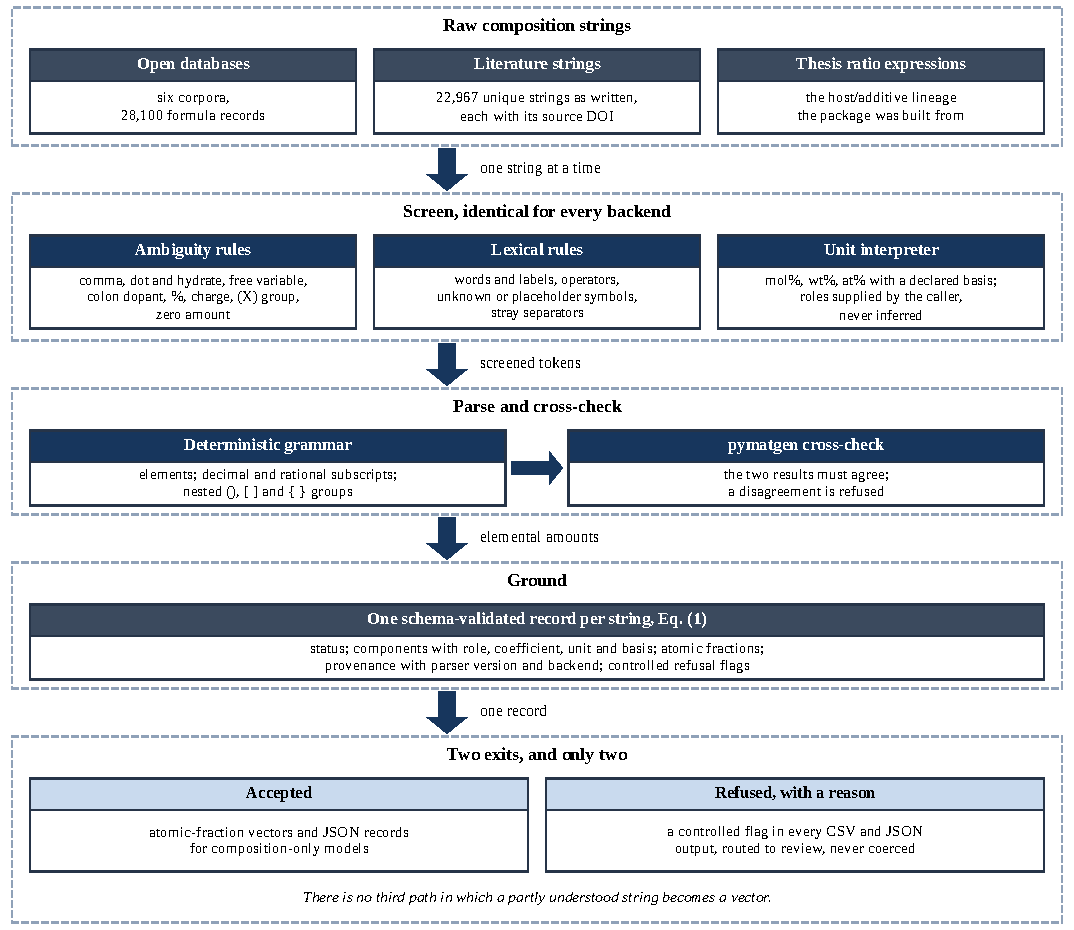
\includegraphics[width=\textwidth]{fig_pipeline_v02.pdf}
\caption{The composition-normalization pipeline. The screen and the grammar fix the accepted language independently of the installed backend; \pmg is used only to check the grammar's result.}
\label{fig:pipeline}
\end{figure*}

The paper's claims are deliberately narrow. It presents a parser artifact and a catalogue of notation hazards observed in published composition strings. The evaluation compares the parser with the composition that an independent text-mining pipeline assigned to each string~\cite{kononova2019textmined}. That reference was produced by another group, but it is a machine reference and not an expert label, and Section~\ref{sec:lit_dev} documents cases in which it is itself wrong. The paper therefore reports agreement with, and discordance from, that reference. It does not report an accuracy or a silent-mis-parse rate for any parser on the doped-ceramic literature.

Refusal has a cost in coverage, and most of that cost on literature strings comes from words around a formula rather than from ambiguous notation: \texttt{Perovskite La0.8Sr0.2MnO3} or \texttt{Mn0.6Zn0.4Fe2O4 MNPs} are refused although the formula inside them is plain. The revision therefore adds an optional normalization stage that removes such words under strict conditions and then hands the residual to the unchanged parser (Section~\ref{sec:stage}). It was designed on the development release and tested twice on held-out strings under a pre-registered rule that allowed no wrong read. It raised agreement with the reference in both tests and failed the safety part of the rule in both. We report both outcomes, and we treat the strings it misread as new entries in the hazard catalogue.

\subsection{Objective}
\label{sec:objective}
The objective is to make composition normalization for doped ceramics auditable, so that for every input string a user can see whether it was resolved or refused and on what grounds. Four specific objectives follow.
\begin{enumerate}
\item O1: Fix the accepted language. Specify, independently of any installed library, which strings resolve and which are refused, and with which controlled reason.
\item O2: Make every output auditable. Validate every record and every tabular output against one schema, with caller-supplied component roles and declared percentage bases.
\item O3: Evaluate on strings as written. Compare the parser and its alternatives on composition strings taken from the literature, against a reference built by another group, with a held-out set that played no part in designing the refusal rules.
\item O4: Name the hazards. Catalogue the notation classes on which an unguarded parser returns a composition that the string does not determine.
\end{enumerate}

\subsection{Contributions}
\label{sec:contributions}
The contributions of this study are as follows.
\begin{enumerate}
\item A deterministic parser (package v\ParserVersion) whose shared lexical screen applies \NFlags{} controlled refusal flags and whose grammar resolves decimal and rational subscripts and nested (), [ ] and \{\,\} groups. \pmg checks each result and never decides what is accepted (O1).
\item A record schema, version 1.1.0, enforced on every output path, including the CSV files. Roles are supplied by the caller and never inferred, and every percentage unit carries a named basis with a closed-form conversion (O2).
\item A literature evaluation on \NLitStrings{} unique strings from two public releases, in which the as-submitted v0.1.0 package, its fallback grammar alone, the v0.2.0 grammar alone, the v0.2.0 package and raw \pmg are each reported separately (O3).
\item An optional normalization stage, run only on refused strings, with five controlled normalization flags and two guards. On two held-out sets it agrees with the reference on \StOneGainPmg{} and \StTwoGainPmg{} more determinate strings than raw \pmg, and it adds no reference-discordant return. Its wrong-read rate among recovered strings is reported with an interval (O3).
\item A catalogue of \NHazClasses{} classes of candidate notation hazards that raw \pmg resolves without a diagnostic, with counts in both releases and a sourced example of each, and two further classes that appear once descriptor words are removed. The benchmark files, the per-string outcomes and the samples prepared for independent expert annotation are released with it (O4).
\end{enumerate}

This study does not claim a general accuracy advantage over \pmg, and its reference is not expert-curated. On the held-out set, the difference between the package and raw \pmg outside the placeholder-symbol class rests on two strings ($p\HoMcDiscExDummyPmgP$, Section~\ref{sec:lit_ho}). The normalization stage gains coverage, but it did not meet its own safety criterion, and the guards added after each test have not been tested on strings their designer had not seen.

\subsection{Organization of the Paper}
\label{sec:organization}
Section~\ref{sec:related} reviews composition parsing and extraction. Section~\ref{sec:method} specifies the record model, the screen, the grammar, the backend policy, the mixture and unit semantics and the schema. Section~\ref{sec:setup} describes the corpora, the benchmarks and the comparison design. Section~\ref{sec:results} reports the results, Section~\ref{sec:limitations} states the limitations, Section~\ref{sec:repro} documents reproducibility and availability, and Section~\ref{sec:conclusion} concludes.

\section{Related Work}
\label{sec:related}
Formula parsing is well served by \pmg~\cite{pymatgen2013,pymatgen2026}, whose \texttt{Composition} object resolves element symbols, brackets and fractional subscripts into element--amount maps. For use with anonymized and defect structures it also accepts non-element \texttt{DummySpecies}, such as \texttt{Xx} or a placeholder \texttt{M}, as valid species~\cite{pymatgen2026}. That behaviour is intended, and it matters here only because a record restricted to real elements must not inherit it. The composition converters of matminer, including \texttt{StrToComposition}, wrap \texttt{Composition}~\cite{ward2018matminer} and therefore share its accepted language. Chemistry has long fixed canonical serializations for structures and molecules, through CIF, SMILES and InChI~\cite{hall1991cif,weininger1988smiles,heller2015inchi}, but no comparable canonical form exists for doped-ceramic mixture notation. That gap is the underlying reason parsing it is hard. FAIR data exchange is advanced by the OPTIMADE API~\cite{optimade2024} and by the wider FAIR programme in materials science~\cite{wilkinson2016fair,draxl2018nomad,scheffler2022fair}. Most machine-readable composition strings come from large computed repositories such as Materials Project, AFLOW, OQMD, JARVIS, Materials Cloud and the Crystallography Open Database, each of which normalizes formulas upstream of any parser~\cite{jain2013mp,curtarolo2012aflow,kirklin2015oqmd,choudhary2020jarvis,talirz2020materialscloud,grazulis2012cod}. Composition-only property models such as CrabNet~\cite{crabnet2021} and Roost~\cite{roost2020}, and the descriptor frameworks before them~\cite{ward2016general,ward2018matminer,dunn2020matbench}, consume the element-fraction vectors that this normalization step produces.

A parallel line of work extracts materials data from the literature. ChemDataExtractor and its successors parse chemical and property mentions from articles and tables~\cite{swain2016chemdataextractor,chemdataextractor2021}, Snowball~2.0 learns extraction patterns~\cite{snowball2023}, and chemical named-entity recognition has a long evaluation tradition~\cite{krallinger2015chemdner}. Domain language models such as MatSciBERT~\cite{matscibert2022} and MaterialBERT~\cite{materialbert2022}, built on SciBERT and BERT~\cite{beltagy2019scibert,devlin2019bert}, improve entity and relation extraction, and benchmarks such as MatSci-NLP~\cite{matscinlp2023} and HoneyBee~\cite{honeybee2023} evaluate them; word embeddings trained on the literature already encode materials knowledge~\cite{tshitoyan2019embeddings}. Text-mined corpora of synthesis recipes are a product of this pipeline~\cite{kononova2019textmined,olivetti2020nlp}. The Kononova et al. release records, for each target material, the string as written, its DOI and the composition that the group's material parser assigned, including variables and dopants~\cite{kononova2019textmined,textminedrepo2023}. That assignment is the reference used in Section~\ref{sec:setup}. Weston et al. normalize recognized material mentions to canonical formulas~\cite{weston2019ner}, and a review of text mining in materials research names punctuation inside formulas, doping notation and abbreviations among the main difficulties of formula extraction~\cite{kononova2021opportunities}. The parser presented here sits downstream of such extractors: it does not locate composition mentions in text, it decides what an extracted string determines.

Machine-actionable records need an agreed model. OPTIMADE defines a database-facing composition and structure schema~\cite{optimade2024}, ChemDataExtractor~2.0 populates hierarchical property records~\cite{chemdataextractor2021}, and MatSci-NLP frames extraction as text-to-schema modelling~\cite{matscinlp2023}. The record model here is narrower: one JSON Schema~\cite{jsonschema2020} for a composition expression, with controlled status and flag vocabularies, explicit roles and unit bases, and provenance, in the spirit of evaluated rather than asserted FAIR metadata~\cite{jacobsen2020interpretations,wilkinson2019maturity,gebru2021datasheets,himanen2019datadriven}. Table~\ref{tab:approach_comparison} compares the approaches on what each one does with notation that does not determine a composition.

\begin{table*}[!t]
\centering
\caption{Composition parsing and representation approaches, compared by behaviour rather than by rating. The entries for \pmg and this package are measured in Section~\ref{sec:results}.}
\label{tab:approach_comparison}
\footnotesize
\begin{tabular}{@{}p{3.0cm}p{3.4cm}p{3.9cm}p{2.7cm}p{2.8cm}@{}}
\toprule
Approach & Accepted formula syntax & Undetermined notation & Percentage units & Output \\
\midrule
\pmg \texttt{Composition} & symbols, decimals, (), [ ] & resolves several classes silently (Table~\ref{tab:hazards}) & not handled & composition object \\
matminer \texttt{StrToComposition} & as \pmg (wraps it) & as \pmg & not handled & composition features \\
Text-mining material parsers & formulas, variables, dopants & assigns variables and additives & partly & extracted records with DOI \\
OPTIMADE schema & not a parser & -- & -- & database records \\
This package (v\ParserVersion) & symbols, decimal and rational subscripts, (), [ ], \{\,\} & refused with \NFlags{} controlled flags & mol\%, wt\%, at\% with declared basis & schema-validated records \\
\bottomrule
\end{tabular}
\end{table*}

\section{Proposed Methodology}
\label{sec:method}

\subsection{Record Model}
\label{sec:record}
Every input expression, resolved or refused, is mapped to one record
\begin{equation}
\label{eq:record}
r = \bigl(f_{\mathrm{raw}},\; s,\; C,\; \phi,\; F,\; \pi\bigr),
\end{equation}
where $f_{\mathrm{raw}}$ is the expression as received (\texttt{raw\_expression}) and $s\in S$ is the parse status (\texttt{parse\_status}), drawn from six controlled states. $C$ is the list of components (\texttt{components}). Each component $(\rho, \sigma, f, c, u, b)$ carries a role $\rho$ (host, additive, dopant, alloying species, solvent or unknown), the source $\sigma$ of that role, a formula $f$, a coefficient $c$ (for a percentage specification, formula units per formula unit of host; otherwise the coefficient as stated), a unit $u$ and, for a percentage, its basis $b$. $\phi$ is the vector of atomic fractions (\texttt{atomic\_fractions}), $F\subseteq V_F$ is the set of refusal flags (\texttt{ambiguity\_flags}) from the \NFlags{}-element vocabulary of Table~\ref{tab:rules}, and $\pi$ is the provenance block (\texttt{provenance}), which always records the parser version and the backend attribution. Two constraints tie the fields together: a resolved record has $F=\emptyset$ and non-empty $C$ and $\phi$, and a refusal has $F\neq\emptyset$ and empty $C$ and $\phi$. The schema states each field and both constraints, and Section~\ref{sec:schema} describes how they are enforced.

\subsection{Shared Lexical Screen}
\label{sec:screen}
The screen applies every refusal rule that does not need a parse, and it runs before the grammar and before \pmg, so the strings the package accepts do not depend on which backend is installed. Table~\ref{tab:rules} lists the rules. A refusal carries every flag that applies, and each flag belongs to one of three status classes. A string is \texttt{ambiguous\_rejected} when it does not determine a composition, \texttt{unsupported\_rejected} when it may determine one but is not a single formula in this grammar, and \texttt{parse\_error} when it is malformed.

\begin{table*}[!t]
\centering
\caption{The shared screen and grammar refusals, with their controlled flag and status class (A: \texttt{ambiguous\_rejected}, the string does not determine a composition; U: \texttt{unsupported\_rejected}, not a single formula in this grammar; E: \texttt{parse\_error}). A refusal carries every flag that applies, not only the first.}
\label{tab:rules}
\footnotesize
\setlength{\tabcolsep}{4pt}
\begin{tabular}{@{}lcp{8.2cm}l@{}}
\toprule
Flag & Class & Trigger & Example \\
\midrule
\texttt{comma\_site\_fraction\_missing} & A & any comma & \texttt{(Ba,Sr)TiO3} \\
\texttt{hydration\_or\_dot\_notation} & A & middle dot; \texttt{.nH2O}; a dot not preceded by a digit (unless followed by 0) & \texttt{Li2O.2SiO2} \\
\texttt{free\_variable\_stoichiometry} & A & x, y, z, $\delta$, $\pm$ outside an element symbol & \texttt{Ba1-xSrxTiO3} \\
\texttt{dopant\_convention\_missing} & A & a colon & \texttt{Y2O3:Eu} \\
\texttt{unit\_convention\_missing} & A & a percent sign; at\% without a count convention & \texttt{CaSc2O4:1\%Ce3+} \\
\texttt{charge\_balance\_unspecified} & A & element, digits, then a sign & \texttt{Ba2+Ti4+O3} \\
\texttt{single\_element\_group} & A & a group holding one bare symbol, no multiplier & \texttt{La(Sr)GaO3} \\
\texttt{nonpositive\_amount} & A & a zero subscript or multiplier & \texttt{BaW0} \\
\texttt{mixture\_or\_arithmetic\_notation} & U & +, -, =, /, \textasciicircum, \textasciitilde{} outside a rational subscript; a leading coefficient & \texttt{BaO-2SiO2} \\
\texttt{non\_formula\_word} & U & lower-case letters outside symbols; a space separating words or phases & \texttt{Pt Nb2O5} \\
\texttt{unknown\_element\_symbol} & U & a capitalised token not among the 118 symbols (incl. D, T, M, Ln, Xx) & \texttt{MS2} \\
\texttt{unconsumed\_separator} & U & any other character, e.g.\ \texttt{@} & \texttt{CdS@ZrO2} \\
\texttt{malformed\_grouping} & E & unmatched or mismatched brackets & \texttt{Ba(Ti0.9Zr0.1]O3} \\
\texttt{backend\_disagreement} & E & grammar and \texttt{pymatgen} return different compositions & -- \\
\texttt{manual\_validation\_required} & E & empty input or no element & -- \\
\bottomrule
\end{tabular}
\end{table*}


Three rules need a justification beyond their trigger. The dot rule refuses a dot that is not preceded by a digit, because \texttt{Ba.9Sr.1TiO3} (a leading-dot decimal) and \texttt{CaO.6Fe2O3} (an adduct, CaO$\cdot$6Fe$_2$O$_3$) have the same form and the string does not say which is meant. A leading dot followed by a zero, as in \texttt{Bi.02}, is accepted, because an adduct multiplier never begins with zero. The space rule accepts whitespace only where it cannot separate two words or two phases: before a subscript (\texttt{Pr 0.6 Sr 0.4 MnO}), after a bare subscript, or between one element symbol and a bracketed group (\texttt{Ba (Bi0.5Nb0.5)O3}). It refuses \texttt{Pt Nb2O5}, \texttt{BaO B2O3 P2O5} and \texttt{CP Cu3Mo6S8}, in which the space may separate phases or a label. The single-element-group rule refuses \texttt{La(Sr)GaO3}, in which the parenthesized symbol marks a dopant of unstated amount rather than one atom of strontium.

\subsection{The Deterministic Grammar}
\label{sec:grammar}
After the screen the grammar is total over the tokens it receives. In EBNF, with $E$ an element symbol among the 118 recognized by IUPAC~\cite{ohrstrom2016elements}:
\begin{align*}
\mathit{Formula} &::= \mathit{Unit}\,\{\mathit{Unit}\}\\
\mathit{Unit}    &::= \mathit{Atom} \mid \mathit{Group}\\
\mathit{Atom}    &::= E\,[\mathit{Number}]\\
\mathit{Group}   &::= \mathit{Open}\;\mathit{Unit}\,\{\mathit{Unit}\}\;\mathit{Close}\,[\mathit{Number}]\\
\mathit{Number}  &::= \mathit{Int}\;\texttt{/}\;\mathit{Int} \mid \mathit{Int}\;\texttt{.}\;\mathit{Int} \mid \texttt{.}\;\mathit{Int} \mid \mathit{Int}\\
\mathit{Open}    &::= \texttt{(} \mid \texttt{[} \mid \texttt{\{} \qquad \mathit{Close} ::= \texttt{)} \mid \texttt{]} \mid \texttt{\}}
\end{align*}
A closing bracket must match the type of the bracket it closes. An omitted number denotes 1, an element contributes its amount to the enclosing scope, and a group contributes each amount of its body multiplied by its own number. Groups nest to any depth, so \texttt{Pb[(Zn0.6Mg0.4)1/3Nb2/3]O3} resolves to Pb$_1$Zn$_{0.2}$Mg$_{0.133}$Nb$_{0.667}$O$_3$. Repeated symbols accumulate, so \texttt{InInO3} and \texttt{In2O3} yield the same amounts. Rational subscripts such as \texttt{La2/3Sr1/3MnO3}, which \pmg does not parse, are part of the grammar. A zero amount or multiplier is refused rather than dropped, because \texttt{BaW0} is far more likely a typing error for BaWO$_4$ than a statement that the compound contains no tungsten.

Fig.~\ref{fig:screen} traces five strings from the development corpus through the screen, the grammar and the cross-check. It shows a string that resolves through both backends, one that only the grammar resolves, and three that are refused.

\begin{figure*}[!t]
\centering
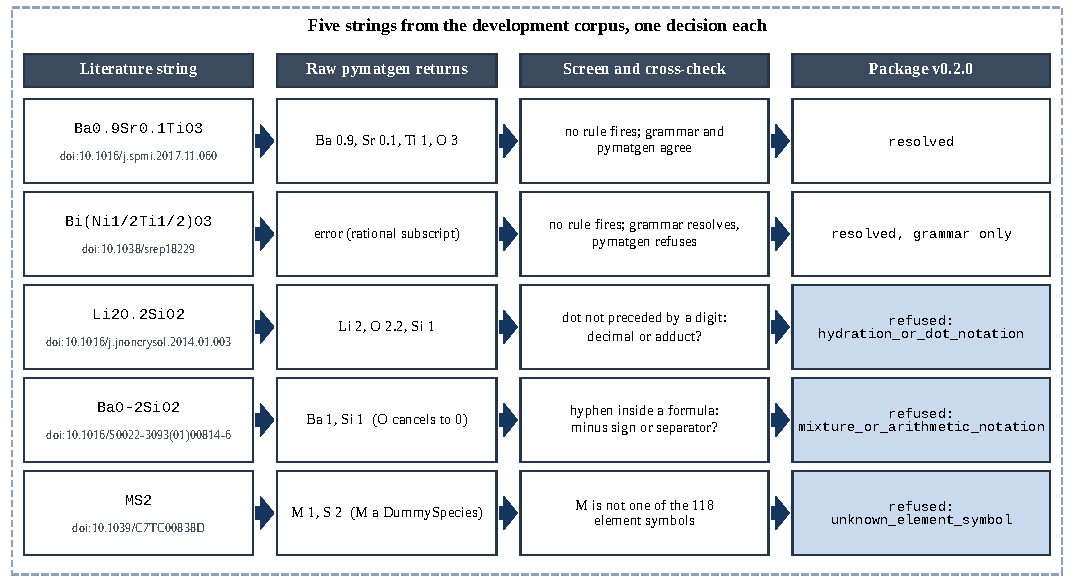
\includegraphics[width=\textwidth]{fig_screen_examples.pdf}
\caption{Five literature strings through the screen, grammar and cross-check. The last three are among the hazard classes of Table~\ref{tab:hazards}; raw \pmg returns a composition for each of them with no diagnostic.}
\label{fig:screen}
\end{figure*}

\subsection{Backend Policy}
\label{sec:backend}
The grammar produces the result. When \pmg is installed, the package also parses the whitespace-stripped string with \texttt{Composition} and compares the two. If both resolve and their atomic fractions differ, the string is refused with \texttt{backend\_disagreement}. If \pmg refuses a string that the grammar resolves, as it does for rational subscripts, the grammar result is returned and attributed as grammar-only. Every record names its backend attribution: \texttt{grammar+pymatgen\_agree}, \texttt{grammar\_only\_pymatgen\_refused} or \texttt{grammar\_only\_pymatgen\_unavailable}. Under this policy the accepted language is the same with or without \pmg, and the cross-check can only add refusals. The submitted version, v0.1.0, preferred \pmg and fell back to its own grammar only when \pmg was absent, applying two shared guards (comma and hydrate) and an element-symbol check to the \pmg result. Its accepted language therefore depended on the installation. Section~\ref{sec:results} reports v0.1.0 unchanged, as a separate configuration.

\subsection{Mixture Expressions and Role Assignment}
\label{sec:mixture}
A mixture expression such as \texttt{0.98BaTiO3+0.02Y2O3} is split at top-level \texttt{+} signs into coefficient--formula terms, and each formula is parsed as above. A hyphen is accepted as a separator only when the caller opts in, every term carries an explicit coefficient, and the coefficients sum to one within $10^{-6}$. Otherwise a hyphen cannot be told apart from a minus sign inside a subscript (\texttt{Ba1-xSrxTiO3}) or from a ratio written without a unit sum (\texttt{BaO-2SiO2}).

Roles are never inferred from the expression. A caller either supplies the role of each component, recorded as \texttt{caller\_supplied}, or opts into the single named rule that the component with the largest coefficient is the host, recorded as \texttt{rule:largest\_coefficient\_is\_host}; a tie under that rule is refused. If the caller does neither, every component has the role \texttt{unknown} with source \texttt{unassigned}. A percentage specification (Section~\ref{sec:units}) is host-plus-additives by construction, because the caller names the host. The role labels in a record are therefore reproducible from the call that produced it.

\subsection{Unit Semantics}
\label{sec:units}
Percentages are semantic operators, not formula tokens, and the same symbol is used in the literature on more than one basis. Every conversion therefore requires the caller to declare the unit, the basis and, for at\%, what is counted, and nothing is defaulted. Let $p_i$ be the stated percentage of additive $i$ divided by 100 and $P=\sum_j p_j$. Let $a$ be the number of atoms per formula unit, $M$ the molar mass, and $\nu_i$ the amount of the named dopant element in one formula unit of additive $i$. Each conversion returns the additive-to-host formula-unit ratio $r_i=n_i/n_H$, as listed in Table~\ref{tab:conventions}.

\begin{table}[!t]
\centering
\caption{Percentage conventions and their closed forms, $r_i=n_i/n_H$. For at\% counting dopant atoms on the total basis, $T=a_H/\bigl(1-\sum_j a_j p_j/\nu_j\bigr)$ is the total number of atoms in the mixture per formula unit of host.}
\label{tab:conventions}
\footnotesize
\renewcommand{\arraystretch}{1.6}
\begin{tabular}{@{}llll@{}}
\toprule
Unit & Counts & Total basis & Per-host basis \\
\midrule
mol\% & formula units & $\dfrac{p_i}{1-P}$ & $p_i$ \\
wt\% & mass & $\dfrac{p_i/M_i}{(1-P)/M_H}$ & $\dfrac{p_i M_H}{M_i}$ \\
at\% & additive atoms & $\dfrac{p_i\,a_H}{(1-P)\,a_i}$ & $\dfrac{p_i\,a_H}{a_i}$ \\
at\% & dopant atoms & $\dfrac{p_i\,T}{\nu_i}$ & $\dfrac{p_i\,a_H}{\nu_i}$ \\
\bottomrule
\end{tabular}
\end{table}

``Total'' means that the percentage is of the whole mixture and ``per host'' that it is relative to the host alone. The at\% convention that counts dopant atoms requires the dopant element to occur in no other component, and otherwise the conversion is refused with \texttt{unit\_convention\_missing}. The same flag is raised for an at\% specification that names no count convention. Molar masses are taken from \pmg's element data. The layer handles any number of additives with formula-unit semantics; it does not infer site occupancy, charge compensation or sublattice-specific at\%.

\subsection{Schema and Output Paths}
\label{sec:schema}
The record schema is a JSON Schema, draft 2020-12~\cite{jsonschema2020}, versioned 1.1.0 and shipped with the package. It defines the fields of Eq.~\eqref{eq:record}, the controlled vocabularies for status, role, role source, unit, basis, at\% count convention, backend attribution and flags, and the two conditional constraints of Section~\ref{sec:record}. A record builder exists for each of the three input forms (a formula, a mixture expression, and a host with percentage additives). Each builder returns a record and never raises on an unparseable string, and the package validates every record it builds. The tabular outputs use the same vocabulary: each CSV row that the package writes carries the controlled status and flags, and no output contains an exception class name. The test suite checks this on every committed output file, and it checks that deliberately corrupted records fail validation. Fig.~\ref{fig:schema} shows the record model and the slots that two worked strings bind. The schema is a record model with controlled vocabularies, not an ontology, and its provenance block admits additional fields, so a valid record is not necessarily a complete one.

\begin{figure*}[!t]
\centering
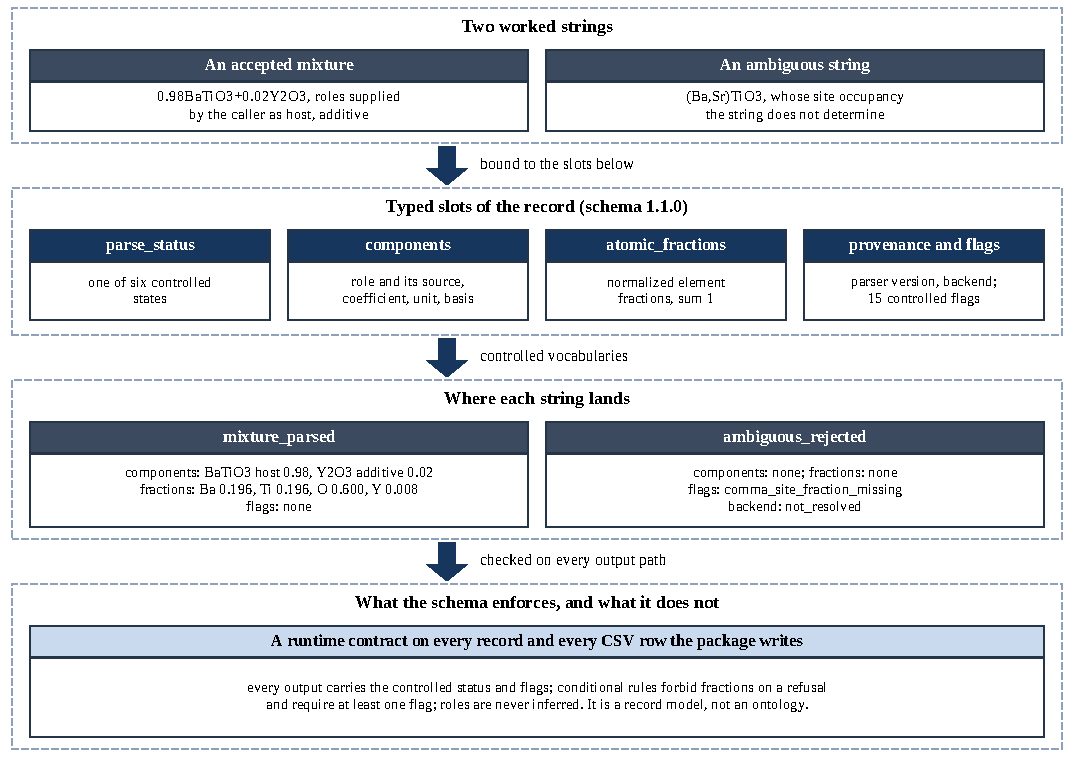
\includegraphics[width=\textwidth]{fig_schema_v02.pdf}
\caption{The \texttt{CeramicCompositionRecord} schema (version 1.1.0) and its grounding relations: two worked strings, the typed slots each binds, and what the schema enforces. A JSON example of each record type is given in ESI Section~S2.}
\label{fig:schema}
\end{figure*}

\subsection{Optional Normalization Stage}
\label{sec:stage}
The stage is a separate module and a separate configuration. It runs only on a string that the v\ParserVersion{} package has refused, and it never changes a string the package resolves. It removes four kinds of text that carry no composition. The first is descriptor words from a closed lexicon: structure types such as \emph{perovskite}, forms such as \emph{nanoparticles} or \emph{MNPs}, chemical-class words such as \emph{oxide} or \emph{titanate}, and element names. The others are a polymorph prefix before a formula ($\alpha$-, $\gamma$-, \texttt{c-}), a thermodynamic state label such as \texttt{(s)}, and stray punctuation left by sentence splitting, such as the bracket and comma in \texttt{(BiFeO3,}. Crystallographic standard uncertainties are also removed, so \texttt{0.13(2)} becomes 0.13. The residual then passes through the unchanged screen, grammar and cross-check. A refusal flag that the residual still raises stands, and every string the stage resolves carries one or more of five normalization flags that record what was removed. The flags are reported beside the composition; they are not yet part of the record schema.

The removal rules are deliberately narrow. A word that qualifies a composition (\emph{doped}, \emph{coated}, \emph{composite}, \emph{rich}, \emph{deficient}, \emph{precursor}, \emph{with}, \emph{and} and similar) blocks the stage for the whole string. A chemical-class word or an element name is removed only if every element it names occurs in the residual formula, so \texttt{silver TiO2} and \texttt{titanate BaZrO3} stay refused. Words may be removed only before or after the formula, never between two formula chunks, and a \texttt{<formula>-type} token is treated as a prototype label. Colons, percentages, slashes, free variables and hyphens other than a polymorph prefix are never touched, so every hazard class of Table~\ref{tab:hazards} keeps its refusal. The residual must contain at least two elements and at least one amount of 1 or more, which stops a fragment such as \texttt{(Ba0.5Sr0.5,} cut out of a longer formula from being read as a whole formula. There is no name-to-formula lookup: a name alone, such as \texttt{barium titanate}, stays refused.

Two guards run on the strings the stage resolves. The first was designed after the first held-out test, on the development release, to catch element lists written as formulas. It refuses a residual with no digit and four or more elements, and it refuses an oxygen-bearing composition that no assignment of the cations' oxidation states can balance within 2\% of the oxygen charge. The states are those that \pmg lists as common or as observed in the Inorganic Crystal Structure Database, and mixed valence is allowed. The second guard was designed after the second held-out test, again on the development release only, to catch a name that contradicts its formula. When a removed word names a salt with a fixed anion charge (nitrate, carbonate, hydroxide, sulfate, phosphate or a halide), the cations at the oxidation states the name implies must balance that charge. When the anion word carries a multiplicity prefix (\emph{dioxide}, \emph{trichloride}), the formula must contain that many anions. When the name states an oxidation state (\emph{iron (III)}, \emph{ferric}), the formula must agree with it. A string refused by either guard keeps its original refusal. The second guard has been checked only on strings its designer had seen (Section~\ref{sec:stage_results}).

\subsection{Use of Generative AI Tools}
\label{sec:ai}
Claude (Anthropic; model \texttt{claude-opus-5-5}) was used in preparing this revision. It drafted code for the revised evaluation and figures, ran the analyses, and drafted revised manuscript text and the response to reviewers. Its prompt was the reviewers' report together with the instruction to revise the paper and package accordingly. In a second round, prompted to test pre-registered improvement hypotheses and to report every outcome, the same tool designed and ran the normalization stage and its guards, wrote the pre-registrations, and made the hand checks of the strings the stage recovered (Section~\ref{sec:stage_design}). Those hand-check labels are the only labels in this paper entered by hand; they are released with a note for every string, and they are not expert labels. The author reviewed, tested and edited all AI-assisted text and code and takes full responsibility for the content, the correctness of the experiments and the released software. Every number in the paper is computed by code from the cited sources or from the released result files.\authoraction{Review the hand-check labels of the 71 and 303 recovered strings (especially the seven wrong reads and the two uncertain ones) before resubmission, and confirm the sentence above.} The tool also drafted the bibliography entries added in this revision, which the author checked against the publisher records.\authoraction{Check the two entries added in the second round (weston2019ner, kononova2021opportunities) against the publisher pages.}\authoraction{Confirm you have checked the new bibliography entries (petousis2017dielectric to jsonschema2020) against the publisher pages.}\authoraction{RSC asks for every tool, version and prompt used across the whole preparation of the work, and for the same disclosure in the cover letter. Add any tools used for the original submission, with versions and prompts, here and in the cover letter.}

\section{Evaluation Design}
\label{sec:setup}

\subsection{Configurations Compared}
Five configurations are run on every input. They are the v0.2.0 package (screen, grammar and cross-check); the v0.2.0 grammar alone, without \pmg; the v0.1.0 package exactly as submitted, with \pmg preferred; the v0.1.0 fallback grammar alone, forced; and raw \pmg~\texttt{Composition} 2026.5.4 with no guards. matminer's \texttt{StrToComposition} is not reported separately, because it wraps \texttt{Composition} and returns the same compositions by construction, as the submitted version confirmed on all \NBench{} hand-written strings; it is therefore not an independent comparator. The two v0.2.0 configurations returned identical results on every input in this study, so most tables show one of them.

\subsection{Database Corpus}
The database corpus is the \NCorpus{} unique (formula, dataset) pairs of six matminer datasets~\cite{ward2018matminer}, comprising \NCorpusDistinct{} distinct formula strings. Table~\ref{tab:provenance} gives, for each dataset, the source publication, the figshare file that matminer retrieves, its SHA-256 digest, the row count and the normalization applied. Of its \NCorpus{} formula records, \NCorpusDecimal{} have decimal subscripts and \NCorpusParen{} (\PctCorpusParen\%) have parentheses, so the corpus exercises almost none of the notation this paper is about. It is used only as a regression check: every configuration must resolve every formula to the same composition.

\begin{table*}[!t]
\centering
\caption{Provenance of the six database corpora: the figshare file identifier and SHA-256 that matminer~0.10.1 records for each named dataset, its row count, and the unique formula strings retained. Normalization: rows with a missing formula are dropped, formulas are compared as exact strings, and duplicate (formula, dataset) pairs are removed; formulas repeated across datasets are kept in each. Dec./Par.: formulas with decimal subscripts / parentheses.}
\label{tab:provenance}
\footnotesize
\setlength{\tabcolsep}{4pt}
\begin{tabular}{@{}llllrrrrr@{}}
\toprule
matminer dataset & Source & figshare file & SHA-256 (first 16) & Rows & Unique & Dec. & Par. & $\bar n_{\mathrm{el}}$ \\
\midrule
\texttt{castelli\_perovskites} & \cite{castelli2012perovskites} & 13284197 & \texttt{fc8b44d7213515f9} & 18{,}928 & 18{,}928 & 0 & 0 & 3.84 \\
\texttt{wolverton\_oxides} & \cite{emery2017perovskites} & 13354616 & \texttt{3e66c2a5bd23dac3} & 4{,}914 & 4{,}914 & 0 & 0 & 2.99 \\
\texttt{double\_perovskites\_gap} & \cite{pilania2016doubleperovskites} & 13309157 & \texttt{746072db995ec46f} & 1{,}306 & 1{,}306 & 0 & 0 & 4.85 \\
\texttt{phonon\_dielectric\_mp} & \cite{petretto2018phonons} & 13297571 & \texttt{53044ba423c06b5c} & 1{,}296 & 1{,}190 & 0 & 72 & 2.91 \\
\texttt{dielectric\_constant} & \cite{petousis2017dielectric} & 13213475 & \texttt{8eb2481214873278} & 1{,}056 & 964 & 0 & 58 & 2.67 \\
\texttt{piezoelectric\_tensor} & \cite{dejong2015piezo} & 13220621 & \texttt{dc9d04836f7f91ec} & 941 & 798 & 0 & 75 & 3.04 \\
\midrule
Total & & & & & 28{,}100 & 0 & 205 & \\
\bottomrule
\end{tabular}
\end{table*}


\subsection{Hand-Written Benchmarks}
Two benchmarks written by the parser's author are retained from the submitted version: a \NStress-string stress test across \NStressFamilies{} notation families, and a \NSeed-row seed set. Both are constructed challenge sets that enumerate notations; they are not samples from any population, so the counts reported for them describe these strings and nothing wider, and no interval is attached to them. Each resolvable string now carries its exact expected element amounts, and a configuration is credited only if it returns those amounts exactly. The labels are those of the submitted version, so no result depends on relabelling. ESI Section~S1 lists all \NBench{} strings with their expected outcomes.

\subsection{Literature Corpora and Reference}
\label{sec:litdesign}
The literature corpora are the two public 2020-07-13 releases of the Kononova et al. text-mined synthesis data~\cite{kononova2019textmined,textminedrepo2023}, fetched from the public repository at a fixed commit and verified by SHA-256. The unit of analysis is the unique target-material string as written in the article, attributed to the first DOI at which it occurs in its release. The development set is the solid-state release, with \NDevStrings{} strings from \NDevDOIs{} DOIs. The held-out set is the sol-gel release, restricted to the \NHoStrings{} strings that do not occur in the solid-state release; they are attributed to \NHoDOIs{} DOIs, \NHoDoiInDev{} of which also occur somewhere in the development release.

Each string is classed from the reference record alone, before any parser runs. A string is \emph{determinate} when the reference assigns a single component whose element amounts are all positive numbers over real element symbols, with no element variable, no oxygen-deficiency marker and no dopant named in the string without an amount. A dopant or a variable value stated elsewhere in the article does not make the string itself indeterminate. A string is a \emph{mixture} when the reference assigns several fully numeric components, and it is \emph{indeterminate} otherwise. Indeterminate strings carry free variables, unquantified dopants, oxygen-deficiency markers or placeholder elements. For each parser and string, the outcome is \emph{agree} (a determinate string resolved to the reference composition, with the same element set and atomic fractions within $10^{-3}$, the precision to which the reference rounds), \emph{disagree} (a different composition for a determinate string), \emph{returned} (a composition for an indeterminate or mixture string) or \emph{refused}. Disagree and returned together are \emph{reference-discordant returns}. They are candidates for silent mis-parses, not confirmed errors, because the reference can itself be wrong.

All refusal rules were designed by inspecting the development set. The held-out evaluation was run once with the parser frozen and its SHA-256 recorded. One rule designed on the development set was then removed before release: it refused a doubled element symbol in a digit-free string, to catch the acronym \texttt{KNN}, but it also refused \NRemovedRuleCorpus{} database formulas such as \texttt{YYOFN}. No held-out outcome changed as a result. Paired differences between configurations are tested with McNemar's exact test~\cite{mcnemar1947}, both with strings as units and, as a sensitivity analysis, with DOIs as units, a DOI counting as discordant if any of its strings is.

\subsection{Evaluation of the Normalization Stage}
\label{sec:stage_design}
The stage was built under a written pre-registration, and so was each guard. Design used the development release only, split by a hash of the DOI into a design half (\StDevHalf{} strings, \StDevHalfDet{} determinate) and a check half (\StDevTestHalf{} strings, \StDevTestHalfDet{} determinate) that could be scored only a fixed, small number of times (three for the stage, two for each guard). The stage file was then frozen by SHA-256 and scored once on held-out strings. The decision rule had three parts, and all three had to hold. First, the stage's count of determinate strings in agreement with the reference had to exceed that of raw \pmg, and that of the v0.1.0 package as submitted (\pmg with an element-symbol check), by at least 3\% of the determinate strings. Second, the exact McNemar test on paired strings had to give $p<0.05$ against both. Third, no wrong read was allowed among the hand-checked recovered strings. A recovered string is one that the stage resolves and the v\ParserVersion{} package refuses. A wrong read is a returned composition that the string, read by a chemist, does not determine. Paired differences carry a 95\% bootstrap interval with DOIs as clusters (4,000 resamples).

The first test used the held-out sol-gel target strings of Section~\ref{sec:litdesign}, with a threshold of \StOneThreshold{} strings, and every recovered string was hand-checked. The first guard was then added, and the second test needed strings that no earlier step had used. Every target string of both releases was already in the development or the held-out set, but the releases also record each precursor as written, with a composition assigned by the same pipeline, and no earlier step had used that field. The second set is the census of unique precursor strings that occur in neither earlier set: \StTwoStrings{} strings from \StTwoDOIs{} first DOIs (\StTwoSolid{} first seen in the solid-state release, \StTwoSolgel{} in the sol-gel release). Their reference classes, computed before any parser ran, are \StTwoDet{} determinate, \StTwoMix{} mixture, mostly hydrates such as \texttt{Fe(NO3)3$\cdot$9H2O}, and \StTwoIndet{} indeterminate. The threshold was \StTwoThreshold{} strings, and the hand check covered a random sample of \StTwoSample{} recovered strings drawn with a fixed seed. Precursors come from the same articles as the targets, so DOIs overlap with both earlier sets and the string, not the DOI, is the unit of independence. Most precursors are simple reagents, which leaves less room for the stage than target strings do.

The hand checks were made with the AI tool of Section~\ref{sec:ai}, not by an independent chemist. The same recovered strings, together with the stratified sample of Section~\ref{sec:limitations}, have been prepared for two independent annotators with a written labelling guide; their labels are pending (Section~\ref{sec:expert}).

\section{Results and Discussion}
\label{sec:results}

\subsection{Database Corpus}
All five configurations resolve all \NCorpus{} database formula records and reproduce the committed atomic-fraction vectors exactly. The corpus therefore cannot separate the configurations, and its perfect parse rate is not evidence about doped-ceramic notation, because the notation the configurations differ on does not occur in it. Its \NCorpus{} records reduce to \NCorpusReduced{} distinct compositions, and \NCorpusCrossDataset{} compositions occur in more than one dataset. ESI Section~S3 gives the element coverage, the per-dataset statistics and the composition-entropy distribution, measured in nats.

\subsection{Hand-Written Benchmarks}
Table~\ref{tab:benchmarks} scores the \NBench{} strings by exact amounts. The v0.1.0 fallback grammar, forced to run alone, returns the exact expected amounts for all \BenchResolvable{} resolvable strings and refuses all \BenchAmbiguous{} ambiguous ones. The v0.1.0 package as submitted returns the same outputs, but in that configuration \pmg, not the grammar, resolved every resolvable string; this table, unlike the submitted version, reports the two separately. The v0.2.0 configurations refuse one string that the benchmark labels resolvable, the leading-dot shorthand \texttt{Ba.9Sr.1TiO3}, under the dot rule of Section~\ref{sec:screen}. The refusal is counted against them, and it is the price of refusing \texttt{Li2O.2SiO2}. Raw \pmg returns compositions for \BenchSilentPmg{} ambiguous strings: \texttt{BaTiO3.2H2O}, \texttt{BaTiO3.H2O} and \texttt{Xx2O3}. The last of these is a mismatch with a schema restricted to real elements, not a parsing error by \pmg, which accepts \texttt{Xx} as a \texttt{DummySpecies} by design.

\begin{table}[!t]
\centering
\caption{The 51 hand-written strings, scored by exact element amounts. $R$: resolvable strings returned with the exact expected amounts; FR: resolvable strings refused (false refusals); $A$: ambiguous strings refused; SM: silent mis-parses (a composition returned for an ambiguous string, or a wrong one for a resolvable string). Labels are those of the submitted version. These are constructed challenge sets, not samples, so no interval is attached to any count. One of raw \texttt{pymatgen}'s three SM, \texttt{Xx2O3}, is a \texttt{DummySpecies} return, a mismatch with a schema restricted to real elements.}
\label{tab:benchmarks}
\footnotesize
\setlength{\tabcolsep}{3pt}
\begin{tabular}{@{}lcccccccc@{}}
\toprule
 & \multicolumn{3}{c}{Stress test (17 + 7)} & \multicolumn{3}{c}{Seed set (21 + 6)} & \multicolumn{2}{c}{Pooled 51} \\
\cmidrule(lr){2-4}\cmidrule(lr){5-7}\cmidrule(l){8-9}
Configuration & $R$ & FR & $A$ & $R$ & FR & $A$ & SM & Correct \\
\midrule
v0.2.0 package & 16 & 1 & 7 & 21 & 0 & 6 & 0 & 50/51 \\
v0.2.0 grammar alone & 16 & 1 & 7 & 21 & 0 & 6 & 0 & 50/51 \\
v0.1.0 as submitted & 17 & 0 & 7 & 21 & 0 & 6 & 0 & 51/51 \\
v0.1.0 grammar alone & 17 & 0 & 7 & 21 & 0 & 6 & 0 & 51/51 \\
raw \texttt{pymatgen} & 17 & 0 & 6 & 21 & 0 & 4 & 3 & 48/51 \\
\bottomrule
\end{tabular}
\end{table}


\subsection{Literature Strings: Development Set}
\label{sec:lit_dev}
Table~\ref{tab:literature} and Fig.~\ref{fig:literature} report the literature evaluation. On the development set, \NDevDet{} of the \NDevStrings{} strings are determinate, \NDevIndet{} indeterminate and \NDevMix{} mixtures. The indeterminate strings are dominated by free-variable subscripts (\DevReasonFreeVar{} strings) and oxygen-deficiency markers (\DevReasonOxDef).

\begin{table*}[!t]
\centering
\caption{Literature strings, by reference class and outcome. Agree: a determinate string resolved to the reference composition (same elements, atomic fractions within $10^{-3}$). Refused: any refusal. Disagree: a composition that differs from a determinate reference. Returned: a composition for a string whose reference is indeterminate or a multi-component mixture. Discordant returns = disagree + returned; they are candidates for silent mis-parses, not confirmed errors (Section~\ref{sec:lit_dev}). Dummy: discordant returns that contain a \texttt{pymatgen} \texttt{DummySpecies}.}
\label{tab:literature}
\footnotesize
\setlength{\tabcolsep}{4pt}
\begin{tabular}{@{}llrrrrrrr@{}}
\toprule
 & & \multicolumn{3}{c}{Determinate} & Indeterminate & Mixture & \multicolumn{2}{c}{Discordant returns} \\
\cmidrule(lr){3-5}\cmidrule(lr){6-6}\cmidrule(lr){7-7}\cmidrule(l){8-9}
Set & Configuration & Agree & Refused & Disagree & Returned & Returned & All & Dummy \\
\midrule
Development ($n=19{,}443$; 7{,}552 / 10{,}518 / 1{,}373) & v0.2.0 package & 6{,}588 & 962 & 2 & 4 & 0 & 6 & 0 \\
 & v0.1.0 as submitted & 6{,}387 & 1{,}155 & 10 & 8 & 4 & 22 & 0 \\
 & v0.1.0 grammar alone & 6{,}303 & 1{,}245 & 4 & 4 & 0 & 8 & 0 \\
 & raw \texttt{pymatgen} & 6{,}387 & 1{,}137 & 28 & 366 & 5 & 399 & 377 \\
\midrule
Held-out ($n=3{,}524$; 1{,}403 / 1{,}889 / 232) & v0.2.0 package & 1{,}099 & 301 & 3 & 0 & 0 & 3 & 0 \\
 & v0.1.0 as submitted & 1{,}096 & 302 & 5 & 0 & 0 & 5 & 0 \\
 & v0.1.0 grammar alone & 1{,}056 & 344 & 3 & 0 & 0 & 3 & 0 \\
 & raw \texttt{pymatgen} & 1{,}098 & 295 & 10 & 43 & 0 & 53 & 48 \\
\bottomrule
\end{tabular}
\end{table*}


\begin{figure*}[!t]
\centering
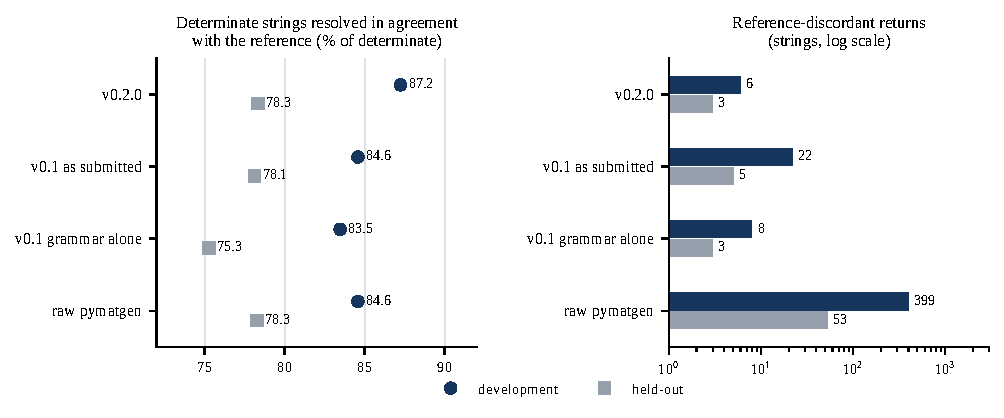
\includegraphics[width=0.92\textwidth]{fig_literature_eval.pdf}
\caption{Literature evaluation. Left: share of determinate strings resolved in agreement with the reference. Right: reference-discordant returns. The v0.2.0 grammar alone coincides with the v0.2.0 package and is not drawn.}
\label{fig:literature}
\end{figure*}

The v0.2.0 package resolves \DevAgreeVtwo{} determinate strings in agreement with the reference (\DevAgreePctVtwo\%), against \DevAgreePmg{} (\DevAgreePctPmg\%) for raw \pmg. In paired terms, it agrees on \DevMcAgreePmgA{} strings where \pmg does not, and \pmg on \DevMcAgreePmgB{} where the package does not ($p\DevMcAgreePmgP$). The gain comes entirely from rational subscripts: every one of the \DevMcAgreePmgA{} strings carries one, which \pmg does not parse, and all resolve through the grammar alone. The cross-check never fired, and grammar and \pmg disagreed on no string that both resolved.

Raw \pmg returns \DevDiscPmg{} reference-discordant compositions, of which \DevDummyPmg{} contain a \texttt{DummySpecies}, against \DevDiscVtwo{} for the package (paired \DevMcDiscPmgA{} versus \DevMcDiscPmgB{}, $p\DevMcDiscPmgP$). Excluding the \texttt{DummySpecies} class, raw \pmg returns \DevDiscExDummyPmg{} and the package \DevDiscExDummyVtwo{} ($p\DevMcDiscExDummyPmgP$; DOI-level $p\DevMcDiscExDummyPmgPDoi$). The v0.1.0 package as submitted removes the \texttt{DummySpecies} returns through its element-symbol check, but otherwise returns the same \DevDiscExDummyVone{} discordant compositions as raw \pmg.

The \DevDiscVtwo{} discordant returns of the package were inspected individually; the list is in the released data. One is a genuine silent mis-parse: the acronym \texttt{KNN}, for K$_{0.5}$Na$_{0.5}$NbO$_3$, is read as KN$_2$, a residual hazard discussed in Section~\ref{sec:limitations}. The other five are reference errors. In \texttt{La0.8Sr0.2Ga0.83Mg0.17O 2.815} the reference discards the spaced oxygen subscript. In four phosphor compositions such as \texttt{La0.9998Sm0.0002Al0.995Cr0.005O3}, the reference rounds a dopant amount of $2\times10^{-4}$ or $3\times10^{-4}$ to zero. This inspection is by the author and is not an independent adjudication.

\subsection{Literature Strings: Held-Out Set}
\label{sec:lit_ho}
On the \NHoStrings{} held-out strings, the package resolves \HoAgreeVtwo{} determinate strings in agreement with the reference (\HoAgreePctVtwo\%) and raw \pmg \HoAgreePmg{} (\HoAgreePctPmg\%); the paired split is \HoMcAgreePmgA{} versus \HoMcAgreePmgB{} ($p\HoMcAgreePmgP$). On these strings the package therefore shows no coverage advantage over \pmg. Raw \pmg returns \HoDiscPmg{} reference-discordant compositions, \HoDummyPmg{} of them containing a \texttt{DummySpecies}, and the package returns \HoDiscVtwo{} ($p\HoMcDiscPmgP$). Outside the \texttt{DummySpecies} class the difference is \HoDiscExDummyPmg{} against \HoDiscExDummyVtwo{}, which on paired strings is \HoMcDiscExDummyPmgA{} versus \HoMcDiscExDummyPmgB{} ($p\HoMcDiscExDummyPmgP$): on held-out data, the evidence that the package returns fewer discordant compositions than \pmg rests on the placeholder class. The package's \HoDiscVtwo{} discordant returns (\texttt{BiFeO 3}, \texttt{LiTi 2}, \texttt{YFeO 3}) share one cause: a subscript separated from its symbol by a space, which the reference discards and the grammar keeps.

\subsection{Normalization Stage on Two Held-Out Sets}
\label{sec:stage_results}
Table~\ref{tab:stage} sets the two held-out tests side by side. In the first, on \StOneDet{} determinate sol-gel target strings, the stage agreed with the reference on \StOneAgree{} (\StOneAgreePct\%), against \HoAgreePmg{} for raw \pmg and \HoAgreeVtwo{} for the package without it. The gain over raw \pmg was \StOneGainPmg{} strings, \StOneDiffPmg{} points (95\% interval \StOneLoPmg{} to \StOneHiPmg), with a paired split of \StOneMcAPmg{} against \StOneMcBPmg{} ($p\StOnePPmg$; with DOIs as units, \StOneDoiAPmg{} against \StOneDoiBPmg, $p\StOnePDoiPmg$). The \StOneMcBPmg{} strings on the other side are the refusal cost of Section~\ref{sec:cost}, which the stage leaves in place. In the second test, on \StTwoDet{} determinate precursor strings, the stage with the first guard gained \StTwoGainPmg{} strings over raw \pmg, \StTwoDiffPmg{} points (\StTwoLoPmg{} to \StTwoHiPmg), split \StTwoMcAPmg{} against \StTwoMcBPmg{} ($p\StTwoPPmg$). Both gains clear the pre-registered thresholds by a wide margin, and both hold against \pmg with the element-symbol check. The agreement levels of the two sets differ widely, \StOneAgreePct\% against \StTwoAgreePctStage\%, because many precursor strings are hydrates and reagent names that every configuration refuses.

\begin{table*}[!t]
\centering
\caption{The optional normalization stage on two held-out sets, each scored once with the stage frozen. Gains are in determinate strings agreeing with the reference, with the paired difference in points and its 95\% DOI-cluster bootstrap interval. McNemar counts are strings that only the stage agrees on against strings that only the comparator agrees on. A recovered string is one the stage resolves and the v\ParserVersion{} package refuses. Wrong reads are from a hand check that is not an expert label; intervals are Wilson 95\% intervals.}
\label{tab:stage}
\footnotesize
\begin{tabular}{@{}lll@{}}
\toprule
 & First test: sol-gel target strings & Second test: unseen precursor strings \\
\midrule
Configuration tested & stage & stage with the first guard \\
Determinate strings & \StOneDet & \StTwoDet \\
Raw \pmg{} agrees & \HoAgreePmg{} (\HoAgreePctPmg\%) & \StTwoAgreePmg{} (\StTwoAgreePctPmg\%) \\
\pmg{} with element check (v0.1.0) agrees & \HoAgreeVone{} (\HoAgreePctVone\%) & \StTwoAgreeVone{} (\StTwoAgreePctVone\%) \\
v\ParserVersion{} package agrees & \HoAgreeVtwo{} (\HoAgreePctVtwo\%) & \StTwoAgreeVtwo{} (\StTwoAgreePctVtwo\%) \\
Stage agrees & \StOneAgree{} (\StOneAgreePct\%) & \StTwoAgreeStage{} (\StTwoAgreePctStage\%) \\
Pre-registered threshold & \StOneThreshold{} strings & \StTwoThreshold{} strings \\
Gain over raw \pmg & $+$\StOneGainPmg; \StOneDiffPmg{} (\StOneLoPmg{} to \StOneHiPmg) & $+$\StTwoGainPmg; \StTwoDiffPmg{} (\StTwoLoPmg{} to \StTwoHiPmg) \\
McNemar against raw \pmg & \StOneMcAPmg{} vs \StOneMcBPmg, $p\StOnePPmg$ & \StTwoMcAPmg{} vs \StTwoMcBPmg, $p\StTwoPPmg$ \\
Gain over \pmg{} with element check & $+$\StOneGainVone; \StOneDiffVone{} (\StOneLoVone{} to \StOneHiVone) & $+$\StTwoGainVone; \StTwoDiffVone{} (\StTwoLoVone{} to \StTwoHiVone) \\
McNemar against \pmg{} with element check & \StOneMcAVone{} vs \StOneMcBVone, $p\StOnePVone$ & \StTwoMcAVone{} vs \StTwoMcBVone, $p\StTwoPVone$ \\
New discordant returns against v\ParserVersion & \StOneNewDiscA & \StTwoNewDiscA \\
Recovered strings, all agreeing with the reference & \StOneRescued & \StTwoRescued \\
Hand-checked & all \StOneRescued & random sample of \StTwoSample \\
Wrong reads & \StOneWrong{} (\StOneWrongPct\%; \StOneWrongLo{} to \StOneWrongHi) & \StTwoWrong{} (\StTwoWrongPct\%; \StTwoWrongLo{} to \StTwoWrongHi) \\
Cause of the wrong reads & element list written as a formula & name contradicts the formula \\
Decision rule, parts 1 / 2 / 3 & pass / pass / fail & pass / pass / fail \\
\bottomrule
\end{tabular}
\end{table*}

Neither test added a reference-discordant return. On every string where the package without the stage returns a composition that the reference contradicts, the stage returns the same one, and every one of the \StOneRescued{} and \StTwoRescued{} recovered strings agrees with the reference. Raw \pmg refuses all of them. In the first test \StOneRescuedOther{} of the \StOneRescued{} came from the stratum of strings with descriptive words or stray punctuation; in the second, \StTwoRescuedOther{} came from that stratum and \StTwoRescuedParen{} from parenthetical strings such as \texttt{Al2O3(s)}.

The safety rule failed both times. The first test found \StOneWrong{} wrong reads among \StOneRescued{} recovered strings, \StOneWrongPct\% (Wilson 95\% interval \StOneWrongLo{} to \StOneWrongHi\%): \texttt{CeGdO oxide}, \texttt{CeZrO2 oxide} and \texttt{VZrPO oxide}. Each lists the elements of a mixed oxide, and \texttt{CeZrO2} cannot be charge-balanced with Ce(IV) and Zr(IV). Two more reads are uncertain, because the prefixes in \texttt{g-La0.8Sr0.2MnO3} and \texttt{sm-LiV3O8} may be processing labels or may not; counting them gives \StOneWrongUPct\% (\StOneWrongULo{} to \StOneWrongUHi\%). The second test, with the guard that targets that class, found \StTwoWrong{} wrong reads in the sample of \StTwoSample, \StTwoWrongPct\% (\StTwoWrongLo{} to \StTwoWrongHi\%): \texttt{strontium nitrate [Sr(NO3)]}, \texttt{tantalum dioxide [Ta2O5]} and \texttt{cobalt hydroxide (Co(OH))2}. A fourth lies outside the sample, \texttt{aluminum nitrate [Al(NO3)2]}, which makes \StTwoWrongAll{} of \StTwoRescued{} overall (\StTwoWrongAllPct\%; \StTwoWrongAllLo{} to \StTwoWrongAllHi\%). In each, the removed name fixes a stoichiometry that the formula contradicts, and the stage checked only that the name's elements occur in the formula. The rate fell between the two tests and its cause changed, but the two sets differ in kind, so the fall cannot be credited to the guard alone. The reference accepts all seven wrong reads.

Applied post hoc to the first test, the first guard refuses the three element-list reads and no other string, which leaves \GuardOneAgree{} in agreement. In the second test it refused \StTwoGuardRefused{} strings in the second test that the unguarded stage returned: \texttt{Na2O1.14(1)}, \texttt{magnesium carbonate [Mg(CO3)2]} and \texttt{strontium nitrate Sr(NO3)3}. The reference agrees with all three, so measured agreement fell by \StTwoGuardCostB{} strings ($p\StTwoGuardCostP$). The last two are names that contradict their formula, and their refusal looks right by hand check. No element-list string appeared among the recovered precursor strings. This test therefore says little about whether the first guard works on its target class.

The second guard was designed on the development release after the second test, and the release contains no recovered string of its target class, so it refused nothing there. No unused pool of literature strings with a reference composition remains in either release: the only other string field, the list of target formulas per reaction, holds formulas generated by the extraction pipeline, none of which contains a word. Its effect can therefore be shown only post hoc, on strings its designer had seen. On the precursor set it refuses exactly the \GthreeTwoRefused{} wrong reads and none of the other recovered strings, and on the target set it refuses nothing. Because the reference accepts the wrong reads, measured agreement on the precursor set falls by \GthreeTwoCost{} strings, to \GthreeTwoAgree{} ($p\GthreeTwoCostP$), and the gain over raw \pmg becomes \GthreeTwoGainPmg{} strings, \GthreeTwoDiffPmg{} points (\GthreeTwoLoPmg{} to \GthreeTwoHiPmg). This shows that the guard does what it was built to do on the cases that motivated it. It is not evidence about its effect on unseen strings.

\subsection{Catalogue of Notation Hazards}
\label{sec:hazards}
Table~\ref{tab:hazards} collects every literature string that raw \pmg resolves without a diagnostic and that the package refuses: \NHazDev{} development and \NHazHo{} held-out strings in \NHazClasses{} classes, each named by its refusal flag. They are candidate hazards, not confirmed errors. In each class the string alone does not settle the reading, or is not a single formula, but \pmg's reading is sometimes the intended one; the leading-dot decimals in the dot class are an example, and the strings counted as refusal cost in Section~\ref{sec:cost} are a subset of this table. Placeholder symbols dominate (for example \texttt{MS2} and \texttt{Ln0.85Ca0.15MnO3}, in which \texttt{M} and \texttt{Ln} stand for an unnamed metal or lanthanide). They are followed by second phases or labels joined across a space (\texttt{Ag CuO}), core--shell composites whose \texttt{@} is ignored (\texttt{CdS@ZrO2}), and parenthesized dopants read as one atom (\texttt{Te(Bi)}). Rarer but chemically severe classes are hyphens read as negative subscripts, which delete the oxide oxygen of \texttt{BaO-2SiO2}, dots read as decimal points, which make \texttt{Li2O.2SiO2} Li$_2$O$_{2.2}$Si and \texttt{FeCl3.6H2O} FeCl$_{3.6}$H$_2$O, and acronyms whose letter T is read as tritium and folded into hydrogen (\texttt{BNT} becomes BNH). The submitted package refused the placeholder symbols through its element-symbol check, but returned compositions for strings in every other class, \NHazVone{} strings in all.

\begin{table*}[!t]
\centering
\caption{Catalogue of candidate notation hazards in the literature corpora: strings that raw \texttt{pymatgen} resolves with no diagnostic and that the v0.2.0 screen refuses, because the string alone does not settle its reading or is not a single formula. They are candidates, not confirmed errors. Classes are named by the v0.2.0 refusal flag. ``v0.1'' counts the strings of the class that the submitted version also returned. The example is the shortest development-set instance; its source is given by DOI.}
\label{tab:hazards}
\footnotesize
\setlength{\tabcolsep}{4pt}
\begin{tabular}{@{}p{4.8cm}rrrlp{3.0cm}p{2.4cm}@{}}
\toprule
Hazard (v0.2.0 flag) & Dev. & Held-out & v0.1 & Example & Source DOI & \texttt{pymatgen} reads \\
\midrule
placeholder symbol accepted as a \texttt{DummySpecies}\newline\texttt{\scriptsize unknown\_element\_symbol} & 362 & 41 & 0 & \texttt{MS2} & {\scriptsize\url{10.1039/C7TC00838D}} & M:1, S:2 \\
label or second phase joined across a space\newline\texttt{\scriptsize non\_formula\_word} & 33 & 18 & 30 & \texttt{Ag CuO} & {\scriptsize\url{10.1016/j.ijhydene.2017.01.105}} & Ag:1, Cu:1, O:1 \\
core--shell or composite \texttt{@} ignored\newline\texttt{\scriptsize unconsumed\_separator} & 7 & 19 & 25 & \texttt{CdS@ZrO2} & {\scriptsize\url{10.1016/j.ultsonch.2017.01.009}} & Cd:1, O:2, S:1, Zr:1 \\
parenthesised dopant read as one atom\newline\texttt{\scriptsize single\_element\_group} & 5 & 3 & 8 & \texttt{Te(Bi)} & {\scriptsize\url{10.1007/s10853-017-1180-9}} & Bi:1, Te:1 \\
zero subscript dropped\newline\texttt{\scriptsize nonpositive\_amount} & 4 & 0 & 4 & \texttt{BaW0} & {\scriptsize\url{10.1016/j.spmi.2015.03.019}} & Ba:1 \\
acronym letter T or D read as hydrogen\newline\texttt{\scriptsize unknown\_element\_symbol} & 4 & 0 & 4 & \texttt{BNT} & {\scriptsize\url{10.1016/j.ceramint.2007.09.098}} & B:1, H:1, N:1 \\
dot read as a decimal point\newline\texttt{\scriptsize hydration\_or\_dot\_notation} & 3 & 2 & 3 & \texttt{Li2O.2SiO2} & {\scriptsize\url{10.1016/j.jnoncrysol.2014.01.003}} & Li:2, O:2.2, Si:1 \\
hyphen read as a negative subscript\newline\texttt{\scriptsize mixture\_or\_arithmetic\_notation} & 3 & 0 & 3 & \texttt{BaO-2SiO2} & {\scriptsize\url{10.1016/S0022-3093(01)00814-6}} & Ba:1, Si:1 \\
\midrule
Total & 421 & 83 & 77 & & & \\
\bottomrule
\end{tabular}
\end{table*}


The normalization stage exposed two further classes (Table~\ref{tab:stage_hazards}). They differ from those of Table~\ref{tab:hazards} in one respect: raw \pmg refuses these strings because of their words, and the hazard appears only once a normalizer removes the words. In the first class a word such as \emph{oxide} or \emph{SiAlON} follows an element list that looks like a formula, so removing the word turns \texttt{CeZrO2 oxide} into a stoichiometry the authors never stated. The same class occurred in the development release, where \texttt{$\alpha$-SiAlON} and \texttt{$\beta$-SiAlON} were read as Si$_1$Al$_1$O$_1$N$_1$; it was noticed only after the first test. In the second class the removed name fixes a stoichiometry that the formula contradicts, as in \texttt{strontium nitrate [Sr(NO3)]}, so the string does not settle which of the two the authors meant. The machine reference accepts every string of both classes. Any pipeline that strips descriptor words before parsing inherits them unless it checks the name against the formula.

\begin{table}[!t]
\centering
\caption{Hazard classes exposed by removing descriptor words. Raw \pmg refuses every string listed; the machine reference accepts every one. ``Wrong read'' strings were returned by the stage tested; ``refused'' strings were refused by the guard given.}
\label{tab:stage_hazards}
\footnotesize
\setlength{\tabcolsep}{3pt}
\begin{tabular}{@{}p{2.2cm}p{3.6cm}p{2.3cm}@{}}
\toprule
Class & Strings & Outcome \\
\midrule
element list written as a formula & \texttt{CeGdO oxide}, \texttt{CeZrO2 oxide}, \texttt{VZrPO oxide} (first test) & wrong read; refused by the first guard (post hoc) \\
 & \texttt{$\alpha$-SiAlON}, \texttt{$\beta$-SiAlON} (development) & wrong read; refused by the first guard \\
\midrule
name contradicts the formula & \texttt{strontium nitrate [Sr(NO3)]}, \texttt{tantalum dioxide [Ta2O5]}, \texttt{cobalt hydroxide (Co(OH))2}, \texttt{aluminum nitrate [Al(NO3)2]} (second test) & wrong read; refused by the second guard (post hoc) \\
 & \texttt{magnesium carbonate [Mg(CO3)2]}, \texttt{strontium nitrate Sr(NO3)3} (second test) & refused by the first guard \\
\bottomrule
\end{tabular}
\end{table}

\subsection{What Refusal Costs}
\label{sec:cost}
A refusal rule also refuses strings that a lenient parser would have resolved correctly. The package refuses \DevCost{} development and \HoCost{} held-out determinate strings that raw \pmg resolves in agreement with the reference. They fall into five groups. The first are core--shell or composite expressions with \texttt{@} (\DevCostAt{} and \HoCostAt). The second are space-separated phases or labels (\DevCostSpace{} and \HoCostSpace). The third are single-element dopant groups (\DevCostGroup{} and \HoCostGroup), the fourth are dot or hydrate forms (\DevCostDot{} plus \DevCostHydrate{}, and \HoCostDot{} plus \HoCostHydrate), and the fifth is a single adduct with a dot after a digit and an unconsumed separator (\HoCostOther{} held-out string, \texttt{CeO2.SiO2}). In most of these the reference shares \pmg's reading rather than confirming it. It records \texttt{FeCl3.6H2O} as FeCl$_{3.6}$H$_2$O and \texttt{Ag CuO} as AgCuO, so agreement between two lenient readings is not evidence that either is right. The cost is nonetheless real for strings such as \texttt{Ba.9Sr.1TiO3}, whose intended reading is clear to a chemist, and for leading-dot decimals such as \texttt{(Lu.999Ce.001)3Al5O12}. All refused strings and their flags are released, so a user who accepts a convention can resolve them explicitly.

\subsection{Expert Labels}
\label{sec:expert}
Two annotators are to label, independently and without parser output, whether each string determines one composition and, if so, which. Their sheets, prepared in this revision, cover the stratified sample of \NAnnotation{} strings and the \StTwoRescued{} strings that the stage recovered in the second test; a written guide fixes the hard cases, including names that disagree with their formula and element lists. Disagreements are adjudicated afterwards, and the original sheets are kept. Inter-annotator agreement is \PENDING{Cohen's kappa, three-class and determinate-or-not, with bootstrap intervals, on the 304-string and 303-string sheets}. On the adjudicated labels, the paired comparison of raw \pmg, \pmg with the element check, the v\ParserVersion{} package and the stage is \PENDING{expert-judged correct returns, wrong returns, correct refusals and refusal costs per parser, with exact McNemar tests}. The departure of the machine reference from the expert labels is \PENDING{reference-versus-expert table}. The stage's wrong-read count on the recovered precursor strings, judged by the annotators rather than by the hand check, is \PENDING{expert-judged wrong reads among the 303 recovered strings}.

\subsection{Mixtures and Unit Semantics}
\label{sec:units_results}
The mixture layer, with the hyphen separator enabled, resolves \DevMixAgree{} of the \NDevMix{} development mixture strings in agreement with the reference and \HoMixAgree{} of the \NHoMix{} held-out ones. It refuses the rest, mostly hyphenated ratios whose coefficients do not sum to one (\texttt{BaO-2SiO2}) or that carry words. Its \DevMixDisagree{} disagreements are reference errors: the reference gives \texttt{0.7TiO2+0.3ZrO2} a zirconium amount of 0.7, and gives \texttt{0.5BiFeO3 + 0.5Bi3.25La0.75Ti3O12} 7.75 oxygen atoms instead of 7.5.

Table~\ref{tab:semantic_unit_eval} shows the unit layer on eight cases with every convention stated, and each ratio is checked in code against the closed form shown. The cases resolve the question that the submitted table left open. For BaTiO$_3$ with Y$_2$O$_3$, 1~mol\% on the total-mixture basis and 1~at\% counting all atoms of the additive phase give the same ratio $r=0.010101$, because both compounds have five atoms per formula unit (cases A1 and A4). The submitted table printed 0.010000 for the mol\% case because it reported the additive's share of all formula units, $x_A=0.01$, rather than $r$. Counting only yttrium atoms changes the answer to $r=0.025641$ (A5), and the per-host basis to $r=0.025$ (A6). Case A8 has two additives.

\begin{table*}[!t]
\centering
\caption{Unit-semantics examples with every convention declared. $r=n_A/n_H$ is the additive-to-host formula-unit ratio (host coefficient 1); $x_A=n_A/(n_H+\sum n)$ is the additive share of all formula units. ``Total'' basis: the percentage is of the whole mixture; ``per host'': of the host alone. For at\%, ``additive atoms'' counts every atom of the additive formula unit and ``dopant atoms'' only the named dopant element. Molar masses for A3: BaTiO$_3$ 233.1922, Y$_2$O$_3$ 225.8099\,g\,mol$^{-1}$. Each $r$ is checked against the closed form shown.}
\label{tab:semantic_unit_eval}
\footnotesize
\setlength{\tabcolsep}{4pt}
\begin{tabular}{@{}lllrlllrr@{}}
\toprule
Case & Host & Additive & \% & Unit & Basis & at\% counts & Derivation of $r$ & $r$ \\
\midrule
A1 & BaTiO$_{3}$ & Y$_{2}$O$_{3}$ & 1 & mol\% & total & -- & \texttt{0.01/(1-0.01)} & 0.010101 \\
A2 & BaTiO$_{3}$ & Y$_{2}$O$_{3}$ & 1 & mol\% & per host & -- & \texttt{0.01} & 0.010000 \\
A3 & BaTiO$_{3}$ & Y$_{2}$O$_{3}$ & 1 & wt\% & total & -- & \texttt{(0.01/M\_Y2O3)/(0.99/M\_BaTiO3)} & 0.010431 \\
A4 & BaTiO$_{3}$ & Y$_{2}$O$_{3}$ & 1 & at\% & total & additive atoms & \texttt{0.01*5/(0.99*5)} & 0.010101 \\
A5 & BaTiO$_{3}$ & Y$_{2}$O$_{3}$ & 1 & at\% & total & dopant atoms & \texttt{0.01*T/2, T=5/(1-5*0.01/2)} & 0.025641 \\
A6 & BaTiO$_{3}$ & Y$_{2}$O$_{3}$ & 1 & at\% & per host & dopant atoms & \texttt{0.01*5/2} & 0.025000 \\
A7 & BaTiO$_{3}$ & C & 1.9 & mol\% & total & -- & \texttt{0.019/(1-0.019)} & 0.019368 \\
A8 & Al$_{2}$O$_{3}$ & Y$_{2}$O$_{3}$; MgO & 0.5; 0.2 & mol\% & total & -- & \texttt{0.005/0.993; 0.002/0.993} & 0.005035; 0.002014 \\
\bottomrule
\end{tabular}
\end{table*}


\subsection{Thesis-Derived Items}
The package descends from a thesis ratio parser. Its six thesis-derived items, three rule paragraphs, one fully normalized expression, one expression with an ambiguity flag and one workflow description, are reported in ESI Section~S4. The one complete expression, \texttt{0.9977076(BaTiO3)+0.003924(Y2O3)+0.019(C)}, is resolved by the mixture layer to O~0.5977, Ba~0.1985, Ti~0.1985, C~0.0038 and Y~0.0016.

\section{Limitations and Threats to Validity}
\label{sec:limitations}

\subsection{The Reference Is Not a Gold Standard}
The reference composition was assigned by another group's extraction pipeline, independently of this paper's author, but it is a machine reference. Sections~\ref{sec:lit_dev}--\ref{sec:units_results} document reference errors in both directions: discarded spaced subscripts, dopant amounts rounded to zero, dots read as decimals and wrong mixture arithmetic. Agreement with the reference is therefore not accuracy, and reference-discordant returns are candidates rather than errors. The inspection of the package's discordant returns was done by the author. A stratified sample of \NAnnotation{} strings across all notation strata and reference classes is released with blank columns for two independent annotators, and the strings recovered by the normalization stage are released in the same form. Expert labels on these strings, with inter-annotator agreement, turn the comparison into an accuracy estimate on the sample; until they are in, every statement about correctness in this paper rests on the machine reference or on a hand check that is not an expert label (Section~\ref{sec:expert}).

\subsection{Residual Hazards}
Two hazard classes are not detectable from the string alone, and the package resolves them silently. An adduct written with a dot after a digit, such as \texttt{Al2O3.2SiO2}, is syntactically a decimal subscript and resolves to Al$_2$O$_{5.2}$Si. An acronym composed of valid single-letter symbols, such as \texttt{KNN}, is syntactically a formula. A rule refusing doubled symbols in digit-free strings would catch \texttt{KNN} but also refused \NRemovedRuleCorpus{} legitimate database formulas, and was removed. Both classes need context that a string parser does not have.

\subsection{Limits of the Normalization Stage}
The stage failed its own safety criterion in both held-out tests, so it is offered as a separate, opt-in configuration and not as part of the parser's accepted language. Its wrong-read rate among recovered strings was \StOneWrongPct\% and \StTwoWrongPct\% in the two tests, with intervals reaching \StOneWrongHi\% and \StTwoWrongHi\%. Both guards were written after the test that exposed the hazard they target, and both held-out sets are now spent, so neither guard has been tested on strings that its designer had not seen. The hand checks behind the wrong-read counts were not made by an expert. The precursor set shares articles with the target sets, and most precursors are simple reagents, so the second test probes a different part of the notation than the first. A fresh test needs strings from a later text-mined release with both 2020 releases removed, or the expert labels of Section~\ref{sec:expert}. Shorthand that happens to balance, such as a hypothetical \texttt{TiZrO2 oxide}, would pass both guards.

\subsection{Scope of the Corpora}
Both literature releases come from one extraction pipeline, whose entity recognition may itself have altered some strings before they reached the parser. Both releases are also weighted towards inorganic synthesis in general rather than doped ceramics specifically. The held-out set is smaller than the development set, and on it the package's advantage over \pmg outside the placeholder class is not statistically supported. The database corpus contains almost none of the notation the paper studies and serves only as a regression check. The hand-written benchmarks were written by the parser's author and describe only themselves.

\subsection{Scope of the Unit Layer and of the Downstream Illustration}
The unit layer covers formula-unit mixtures with any number of additives. It does not infer site occupancy, charge compensation or sublattice-specific at\%, and it refuses rather than guesses when a count convention is missing. The submitted downstream property check compared atomic-fraction vectors with a character-level string baseline on one dielectric dataset. Every configuration in this study parses those \NDiel{} formulas identically, so the check cannot distinguish parsers and is no longer offered as evidence. ESI Section~S5 reports it as an illustration only, together with a check for leakage across folds: no two records share a reduced composition, but \NDielInSharedSystems{} of the \NDiel{} records share a chemical system with another record. The section also gives the revised protocol, with folds grouped by chemical system and a Magpie baseline.

\section{Reproducibility and Availability}
\label{sec:repro}
The package is the installable distribution \texttt{ceramic-composition-parser}, version \ParserVersion, with schema 1.1.0. The released parser file is identified by its SHA-256 in the archive, as is the frozen version used for the first held-out run. \pmg is pinned to 2026.5.4 (with \texttt{pymatgen-core} 2026.8.30), the versions that produced every reported number, and matminer to 0.10.1. One entry point regenerates every result, table, figure and number in this paper from the committed inputs; each count, percentage and test statistic in the text is a macro written by the code rather than typed. The two literature releases are not redistributed. A fetch script retrieves them from the public repository at commit \texttt{fca0a99} and verifies their SHA-256 digests. The archive contains the per-string outcomes of all five configurations on both releases, the 51 benchmark strings with expected amounts, the annotation samples, and a test suite that checks the parser rules, the schema contract on every output file, and the agreement between the committed results and the generated tables.

The normalization stage is released as two further modules beside the package, with the pre-registrations, the SHA-256 digests recorded before each held-out run, the scoring scripts, the per-string outcomes of both tests and the hand-check labels with a note for every recovered string. Its numbers are written into macros by a script that reads those result files. All of this is in the folder \texttt{normalization\_stage} of the archive and is listed with its SHA-256 digest in the archive manifest. The digest of each stage module in the archive equals the one recorded before its held-out run, and the macro script run on the archived result files reproduces every stage number in this paper.

\depositis{The versioned archive (v\ParserVersion) accompanies this submission as electronic supplementary information. A public deposit with a persistent identifier does not yet exist; it will be created from the same archive and cited here.}{The versioned archive (v\ParserVersion) is deposited at \depositdoilink.}

\section{Conclusion and Future Work}
\label{sec:conclusion}
The paper presents a composition parser whose accepted language is fixed by a shared screen and a deterministic grammar, whose every output is a schema-validated record with controlled refusal reasons, and whose unit conversions state their basis. On literature strings the parser alone does not beat \pmg: held-out coverage of determinate strings is equal, and its lower count of reference-discordant returns comes mostly from placeholder symbols that \pmg accepts by design.

The optional normalization stage is the one change that raised coverage on held-out data. It agreed with the reference on \StOneGainPmg{} and \StTwoGainPmg{} more determinate strings than raw \pmg in two tests, each run once with the stage frozen, and it added no reference-discordant return. It also misread \StOneWrongPct\% and \StTwoWrongPct\% of the strings it recovered, so it failed the zero-wrong-read rule we set for it, and it stays an opt-in candidate. Its failures were informative. They define two hazard classes, element lists written as formulas and names that contradict their formula, that only appear once a normalizer removes words, and that the machine reference accepts. With the \NHazClasses{} classes that \pmg resolves without a diagnostic, they form the catalogue that we regard as the paper's most durable result.

Three things remain open. The expert labels of Section~\ref{sec:expert} will show whether the refusals and the stage's reads are right by a chemist's judgement. The guards need a test on strings no one has seen, which requires a new text-mined release. Contextual rules, such as resolving a placeholder or an acronym from the surrounding text, would address the residual hazards that no string-level rule can see.

\section*{Declarations}

\subsection*{Data Availability}
The database corpora are matminer datasets identified in Table~\ref{tab:provenance}. The literature strings are from the public text-mined synthesis releases of Kononova et al.~\cite{kononova2019textmined,textminedrepo2023}, identified by repository commit and file digest. The benchmark files, the per-string evaluation outputs and the annotation sample are in the archive described in Section~\ref{sec:repro}.

\subsection*{Code Availability}
The parser, the schema, the evaluation code and the tests are in the archive described in Section~\ref{sec:repro}, under the MIT licence. \depositis{The archive accompanies this submission; its public deposit is pending.}{The archive is deposited at \depositdoilink.}\authoraction{Mint the Zenodo DOI for the release archive, set it in deposit_doi.tex, rebuild.}

\subsection*{Funding}
This research received no external funding.

\subsection*{Competing Interests}
The author declares no competing interests.

\subsection*{Author Contributions}
Imran: Conceptualization, Methodology, Software, Validation, Formal analysis, Investigation, Data curation, Writing (original draft), Writing (review and editing), Visualization, Project administration.

\bibliographystyle{IEEEtran}
\bibliography{references}
\end{document}
